\def\topic{SetsLectures}
\def\format{print}

\documentclass[10pt]{memoir}
\chapterstyle{ell}
% Font choices: Euler for math; Palatino for rm; Helvetica for ss; Courier for tt

\typeout{PACKAGES!!!! \format}
\usepackage{etoolbox}
\usepackage[dvipsnames]{xcolor}

\renewcommand{\rmdefault}{ppl} % rm
\linespread{1.05}        % Palatino needs more leading
\usepackage[scaled]{helvet} % ss
\usepackage{courier} % tt
\usepackage{euler} % math
\normalfont
\usepackage[T1]{fontenc}
\usepackage{microtype}



\ifdefstring{\format}{print}{
	\usepackage[letterpaper,
		left=2cm,
		top=1.5cm,
		right=5cm,
		bottom=2cm,
		marginparwidth=4cm,
		marginparsep=3mm]{geometry}

}
{}
\ifdefstring{\format}{ipad}{
	\usepackage[paperwidth=9in,
		paperheight=6in,
        left=3mm,% right=3mm,
        top=1mm,
		bottom=1mm,
		right=3cm]{geometry}
}
{}
\ifdefstring{\format}{kindle}{
	\usepackage[papersize={3.6in,4.8in},
		hmargin=0.1in,
		vmargin={0.1in,0.1in}]{geometry}

}
{}

% Symbols
\usepackage{latexsym,amssymb,amsmath,eucal,times,stmaryrd,bbold}

% Must have tikz
\usepackage{tikz}
\usepackage{hyperref}
\input(bubble.sty)

\IfFileExists{\topic.meta.tex}{\input{\topic.meta.tex}}{}

\newcommand{\setAuthor}[1]{\immediate\write\metafile{\noexpand\def\noexpand\Author{#1}}}
\newcommand{\setTopic}[1]{\immediate\write\metafile{\noexpand\def\noexpand\Topic{#1}}}
\newcommand{\setCourse}[1]{\immediate\write\metafile{\noexpand\def\noexpand\Course{#1}}}
\newcommand{\setDate}[1]{\immediate\write\metafile{\noexpand\def\noexpand\Date{#1}}}
\newcommand{\setVersion}[1]{\immediate\write\metafile{\noexpand\def\noexpand\Version{#1}}}
\newcommand{\setOverview}[1]{\immediate\write\metafile{\noexpand\long\noexpand\def\noexpand\Overview{#1}}}


\AtEndPreamble{\newwrite\metafile\immediate\openout\metafile=\topic.meta.tex}
\AfterEndDocument{
%\immediate\write\metafile{\noexpand\providecommand{\noexpand\Author}{M. A. M.}}
\closeout\metafile
}

\providecommand {\Author }{M. A. Moshier}
\providecommand{\Topic}{Stuff}
\providecommand{\Course}{Discrete Mathematics}
\providecommand{\Date}{\today}
\providecommand{\Version}{0:0.0}
\providecommand{\Overview}{}



\makeatletter
\renewcommand*{\beforepartskip}{\null\vskip4cm}
\renewcommand*{\afterpartskip}{\par\vfil%
\@afterindentfalse\@afterheading}
\makeatother

\def\NN{\mathbb N}
\def\RR{\mathbb R}
\def\CC{\mathbb C}
\def\QQ{\mathbb Q}
\def\ZZ{\mathbb Z}
\def\One{\mathbb 1}
\def\Two{\mathbb 2}
\def\tt{\textsc{t}}
\def\ff{\textsc{f}}

\newcommand{\printbreak}{\iftoggle{printformatting}{\newpage}{}}
\newcommand{\ipadbreak}{\iftoggle{ipadformatting}{\newpage}{}}
\newcommand{\kindlebreak}{\iftoggle{kindleformatting}{\newpage}{}}

\newlength{\proofsep}
\setlength{\proofsep}{1.5\baselineskip}
\newenvironment{proof}{\vskip\proofsep\noindent \textbf{Proof:}\ }{$\Box$}

\newcommand{\id}{\textsf{id}}

\newcommand{\st}{\,\mid\,}

\newcommand{\iso}{\simeq}

\newcommand{\fromto}[3]{{#1}\colon{#2}\to{#3}}
\newcommand{\sfromto}[3]{#2\stackrel{#1}{\longrightarrow}#3}
\newcommand{\powerset}{{\mathcal{P}}}

\makeatletter
\newcommand*{\doublerightarrow}[2]{\mathrel{
  \settowidth{\@tempdima}{$\scriptstyle#1$}
  \settowidth{\@tempdimb}{$\scriptstyle#2$}
  \ifdim\@tempdimb>\@tempdima \@tempdima=\@tempdimb\fi
  \mathop{\vcenter{
    \offinterlineskip\ialign{\hbox to\dimexpr\@tempdima+1em{##}\cr
    \rightarrowfill\cr\noalign{\kern-.2ex}
    \rightarrowfill\cr}}}\limits^{\!#1}_{\!#2}}}
\newcommand*{\doubleleftarrow}[2]{\mathrel{
  \settowidth{\@tempdima}{$\scriptstyle#1$}
  \settowidth{\@tempdimb}{$\scriptstyle#2$}
  \ifdim\@tempdimb>\@tempdima \@tempdima=\@tempdimb\fi
  \mathop{\vcenter{
    \offinterlineskip\ialign{\hbox to\dimexpr\@tempdima+1em{##}\cr
    \leftarrowfill\cr\noalign{\kern.5ex}
    \leftarrowfill\cr}}}\limits^{\!#1}_{\!#2}}}
\makeatother

\newcommand{\symb}[1]{{\mathord{\textsf{#1}}}}
\newcommand{\curry}{\mathord{\textsf{curry}}}
\newcommand{\suc}{\mathord{\textsf{suc}}}
\newcommand{\pred}{\mathord{\textsf{pred}}}

\newcommand{\nxt}{\curvearrowright}
\newcommand{\len}{\mathord{\textsf{len}}}
\newcommand{\map}{\mathord{\textsf{map}}}
\newcommand{\appl}{\mathord{\textsf{appl}}}
\newcommand{\inj}{\mathord{\textsf{inj}}}
\newcommand{\constant}{\mathord{\textsf{c}}}
\newcommand{\List}{\mathord{\textsf{List}}}
\newcommand{\srec}{\mathord{\textsf{s-rec}}}
\newcommand{\primrec}{\mathord{\textsf{p-rec}}}
\newcommand{\rank}{\mathord{\textsf{rank}}}
\newcommand{\suit}{\mathord{\textsf{suit}}}
\newcommand{\size}[1]{{\lVert #1\rVert}}
\newcommand{\ddiv}{\mathop{/\mkern-5mu/}}


\newcommand{\pluseq}{\mathrel{\mathord+\mathord=}}
\newcommand{\minuseq}{\mathrel{\mathord-\mathord=}}
\newcommand{\timeseq}{\mathrel{\mathord*\mathord=}}
\newcommand{\diveq}{\mathrel{\mathord\ddiv\mathord=}}
\newcommand{\modeq}{\mathrel{\mathord\%\mathord=}}
\newcommand{\defeq}{\coloneqq}

\newcommand*{\treewedge}{%
\mathrel{\vcenter{\offinterlineskip
\vskip-2ex\hbox{$\wedge$}}}}

\newcommand{\ignore}[1]{}

\newlist{exerciseslist}{enumerate}{1}
\setlist[exerciseslist]{resume,label=\arabic*.}
\newenvironment{exerciselist}{\begin{exerciseslist}}{\end{exerciseslist}}
%\newenvironment{nextexercise}{\begin{enumerate}[resume=exercises]}{\end{enumerate}}

\newenvironment{goal}[1]{\noindent\textbf{#1}\begin{itemize}}{\end{itemize}}

\makeatletter\@addtoreset{exerciseslisti}{chapter}\makeatother

%\input{style.tex}

\newlength\drop
\newcommand*{\mytitle}{
	\begingroup%
		\drop=0.1\textheight
		\fboxsep 0.5\baselineskip
		\sffamily
		{\centering
			{\Large \Course}\par
			\vspace{0.3\drop}
			{\Large Lecture Notes}\par
			\vspace{0.3\drop}
			{\Large on}\par
			\vspace{0.3\drop}
			{\Large \Topic}\par
			\vspace{0.9\drop}
			{\large \Author}\par
			\vspace{0.3\drop}
			{\Date}\par
			\vspace{1\drop}
		}
		\vfill
		\begin{overview}\Overview\end{overview}\par
		\vfill
	{\small Version: \Version\ (\today) Format: \format}
	\endgroup
}

%\newcommand{\setTopic}[1]{\def\Topic{#1}}
%\newcommand{\Date}{October 2014}
%\newcommand{\Overview}{We will study sets and functions}

%\setTopic{Sets and Functions}

\begin{document}	
\pagestyle{empty} 
\mytitle
\clearpage
\pagestyle{simple}
\tableofcontents
\clearpage

\input{\topic.tex}

%\newwrite\metafile
%\immediate\openout\metafile=meta.tex
%\immediate\write\metafile{\noexpand\providecommand{\noexpand\Author}{M. A. M.}}
%\closeout\metafile

\end{document}

% \part{Introduction}

% Recurring ideas in this course.
% \begin{itemize}
% \item Natural numbers. The natural numbers (counting numbers), without
%   question, constitute the fundamental structure in mathematics.
%   Nearly everything else depends on understanding how natural numbers
%   behave. And yet, you have known how to count from a very young
%   age. So it turns out that a great deal of very sophisticated
%   mathematics depends on us going back to basics, and simply looking
%   carefully at some ideas we already know.
% \item Universal constructions. It turns out that a lot of the ideas in
%   mathematics exhibit a general pattern of being ``universal'' for a
%   particular problem. A simple example is the \emph{floor} of a real
%   number $x$. This is the integer (written $\lfloor x\rfloor$) that is
%   as large as possible and still less than or equal to $x$. So the
%   floor of $5.3$ is $5$ and the floor of $-1.2$ is $-2$.  The floor is
%   universal for the problem of finding an integer $m$ so that $m\leq
%   x$. There are infinitely many integers satisfying this inequality,
%   but $\lfloor x\rfloor$ is the only one we need to know because for
%   an integer, $m\leq x$ is exactly the same as $m\leq \lfloor
%   x\rfloor$.
 
%   Many other constructions that have nothing obvious to do with
%   numbers are similar. A \emph{universal construction} solves a
%   particular problem in such a way that all other solutions are
%   related to the universal construction.
% \item Duality. Many ideas is mathematics come in pairs: minimum and
%   maximum, great common divisor and least common multiple, ``and'' and
%   ``or'', union and intersection. All of these are examples of
%   \emph{duals} concepts. Dual concepts are helpful because a lot of
%   what we can learn about one of a dual pair is automatically true of
%   the other.
% \item Concrete mathematics. We do not shy away from concrete
%   calculations. This will be especially so in the last part of the
%   course.
% \end{itemize}

%\part{Numbers}
% 2
%\chapter{The Natural Numbers}

The \emph{natural numbers} have to do with counting: 0, 1, 2, 3, \ldots.
They do not include negatives
or fractions or irrationals.
In this lecture, the structure of natural numbers is the topic.
To hone in on that structure, we look at structures similar to the natural numbers, but that
fail to capture some basic aspects of counting. Bogus structures
are ruled out by axioms that distinguish the structure of natural numbers
from all others.

\begin{goals}
\noindent \textbf{Lecture}
\begin{itemize}
\item Present the natural numbers as comprising a structure suited to counting.
\item Identify similar structures that can not properly represent counting.
\item Rule out ``bad'' structures via axioms.
\end{itemize}

\noindent \textbf{Study}
\begin{itemize}
\item Gain facility in the course's \emph{successor} notation, including
translating between successor notation and base $10$ notation.
\item Commit to memory the axioms of natural numbers.
\item Demonstrate ability to recognize failures of the axioms. 
\end{itemize}
\end{goals}

\section{The Basic Picture}

Natural numbers are pictured like stepping stones in 
Figure \ref{fig:nat-numbers}.

\begin{figure}[h]
  \centering
  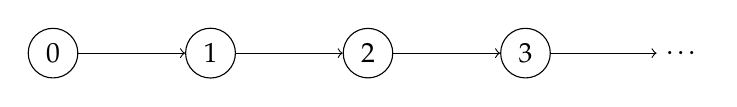
\begin{tikzpicture}
    \node (a) at (0,0) [circle, draw] {0};
    \node (b) at (2,0) [circle,draw] {1}; \node (c) at (4,0)
    [circle,draw] {2}; \node (d) at (6,0) [circle,draw] {3}; \node (e)
    at (8,0) {\ldots}; \draw[->] (a.east) -- (b.west); \draw[->]
    (b.east) -- (c.west); \draw[->] (c.east) -- (d.west); \draw[->]
    (d.east) -- (e.west);
  \end{tikzpicture}
  \caption{A picture of the natural numbers}
  \label{fig:nat-numbers}
\end{figure}

Figures \ref{fig:NatSigBad1}, \ref{fig:NatSigBad2} and \ref{fig:NatSigBad3} illustrate three
ways \emph{not} to picture the natural numbers.

\begin{figure}[h]
\centering
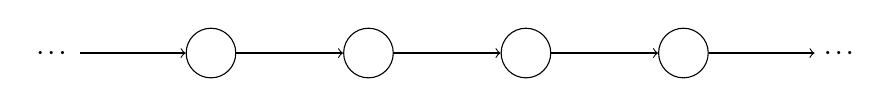
\begin{tikzpicture}
  \node (z) at (-2,0) {\ldots}; 
\node (a) at (0,0) [circle, draw] {\phantom0};
    \node (b) at (2,0) [circle,draw] {\phantom0}; \node (c) at (4,0)
    [circle,draw] {\phantom0}; \node (d) at (6,0) [circle,draw] {\phantom0}; 
    \node (e) at (8,0) {\ldots}; 
    \draw[->] (z.east) -- (a.west); \draw[->] (a.east) -- (b.west); \draw[->]
    (b.east) -- (c.west); \draw[->] (c.east) -- (d.west); \draw[->]
    (d.east) -- (e.west);
%\node (left) at (0,0) [circle,draw] {}; \node (center) at (1,0)
%  [circle,draw] {}; \node (right) at (2,0) [circle,draw] {}; \draw[<-]
%  (left.north east)--(center.north west); \draw[->] (center.south
%  east)--(right.south west); \draw[->] (left.south
%  east)--(center.south west); \draw[<-] (center.north
%  east)--(right.north west);
\end{tikzpicture}
\caption{Nowhere to start}\label{fig:NatSigBad1}

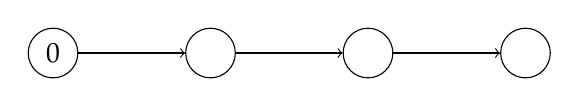
\begin{tikzpicture}
  \node (a) at (1,0) [circle, draw] {0};
    \node (b) at (3,0) [circle,draw] {\phantom0}; \node (c) at (5,0)
    [circle,draw] {\phantom0}; \node (d) at (7,0) [circle,draw] {\phantom0}; 
    \draw[->] (a.east) -- (b.west); \draw[->]
    (b.east) -- (c.west); \draw[->] (c.east) -- (d.west);
\end{tikzpicture}
\caption{Nowhere to go}\label{fig:NatSigBad2}

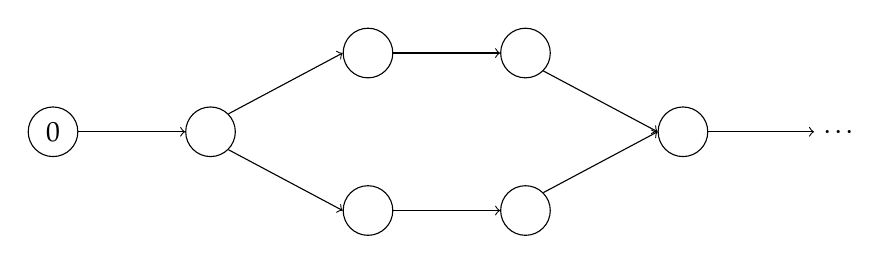
\begin{tikzpicture}
%    \node (a) at (0,0) [circle, draw] {0};
    \node (b) at (2,0) [circle,draw] {0}; 
    \node (c) at (4,0) [circle,draw] {\phantom0}; 
    \node (d1) at (6,1) [circle,draw] {\phantom0}; 
    \node (d2) at (6,-1) [circle,draw] {\phantom0}; 
    \node (e1) at (8,1) [circle,draw] {\phantom0}; 
    \node (e2) at (8,-1) [circle,draw] {\phantom0};
    \node (f) at (10,0) [circle,draw] {\phantom0};
    \node (g) at (12,0) {\ldots};
%    \draw[->] (a.east) -- (b.west); 
    \draw[->] (b.east) -- (c.west); 
\draw[->] (c.north east) -- (d1.west);
\draw[->] (c.south east) -- (d2.west);
\draw[->] (d1.east) -- (e1.west);
\draw[->] (d2.east) -- (e2.west);
\draw[->] (e1.south east) -- (f.west);
\draw[->] (e2.north east) -- (f.west);
\draw[->] (f.east) -- (g.west);
\end{tikzpicture}
\caption{Forks in the path}\label{fig:NatSigBad3}
\end{figure}

These incorrect pictures can be ruled out by explaining the basic structure of counting.

\ipadbreak

%\refstepcounter{axiomCnt}
\begin{signature}{Nat}\label{sig:NatSignature}
The natural numbers have the following basic structure.
  \begin{itemize}
  \item There is a special natural number. We denote this by $0$.
  \item For any natural number $n$, there is
    a unique \emph{next} natural number. We call this the \emph{successor of $n$}. 
    In these lectures, we denote the successor of $n$ by $n^\nxt$.
  \end{itemize}
\end{signature}

%\begin{text-usage}
%	In these notes, bubbles labelled ``Signature'' introduce new notation meant to capture the essential structure of what we are talking about.
%	Here are want to talk about natural numbers as the things we use to count. So the essense is that counting ``starts somewhere'' ($0$) and it ``keeps going'' (any $n$ is followed by $n^\nxt$).
%	Later we will also introduce other notation, for example $+$ for addition and $\leq$ for the greater-than-or-equal-to relation between two numbers. But these are add-ons, not essential to the very idea of counting.
%\end{text-usage}
%
%\begin{usage}
%  The notation $n^\nxt$ is not standard. We will use it in these notes for pedagogical reasons.
%After the first few lectures, we will not need it very often. If you use it in another course, you will need to
%explain it, as it is unlikely that othe professors will know what it means. Clearly, $n^\nxt$ is intended to be the same as $n+1$,
%but we are talking about \emph{counting} not \emph{adding}.
%This notation, in which a natural number is written as $0$ followed by some ${}^\nxt$'s, we will call \emph{successor notation}.  For example,
%$0^{\nxt\nxt\nxt}$ is the successor notation corresponding to the number three.
%\end{usage}

\begin{exercises}
\begin{multicols}{2}
%\begin{itemize}
\item Convert the following to successor notation.
  \begin{enumerate}
  \item $9$
  \item $10$
  \item $4 + 3$
  \item $n + 4$
  \end{enumerate}
\item Convert the following to base $10$ notation.
\begin{enumerate}
\item $0^{\nxt\nxt\nxt\nxt}$
\item $n^{\nxt\nxt\nxt\nxt\nxt}$
\item $5^{\nxt\nxt}$
\item $0^\nxt + 0^{\nxt\nxt}$
\end{enumerate}
%\end{itemize}
\end{multicols}
\end{exercises}

\ipadbreak

\section{Narrowing the possibilities}

Figures \ref{fig:one-loop} and \ref{fig:two-loop} illustrate 
problems that \ref{ax:NatSignature} does not avoid.

\begin{figure}[h]
  \centering
  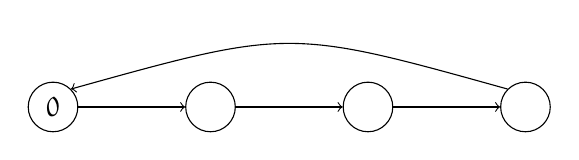
\begin{tikzpicture}
    \node (a) at (0,0) [circle, draw] {$0$}; \node (b) at (2,0)
    [circle,draw] {\phantom{$0$}}; \node (c) at (4,0) [circle,draw]
    {\phantom{$0$}}; \node (d) at (6,0) [circle,draw] {\phantom{$0$}};
    \draw[->] (a.east) -- (b.west); \draw[->] (b.east) -- (c.west);
    \draw[->] (c.east) -- (d.west); \draw[->] (d.north west)
    .. controls (3,1) .. (a.north east);
  \end{tikzpicture}
  \caption{A strange way to count}
  \label{fig:one-loop}
\end{figure}

\begin{figure}[h]
  \centering
  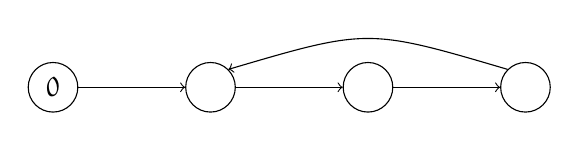
\begin{tikzpicture}
    \node (a) at (0,0) [circle, draw] {$0$}; \node (b) at (2,0)
    [circle,draw] {\phantom{$0$}}; \node (c) at (4,0) [circle,draw]
    {\phantom{$0$}}; \node (d) at (6,0) [circle,draw] {\phantom{$0$}};
    \draw[->] (a.east) -- (b.west); \draw[->] (b.east) -- (c.west);
    \draw[->] (c.east) -- (d.west); \draw[->] (d.north west)
    .. controls (4,.75) .. (b.north east);
  \end{tikzpicture}
  \caption{Another strange way to count}
  \label{fig:two-loop}
\end{figure}

\begin{exercises}
%\begin{itemize}
\item
Explain, in one or two sentences each, why Figures \ref{fig:one-loop} and \ref{fig:two-loop} satisfy Axiom \ref{ax:NatSignature}.
%\end{itemize}
\end{exercises}
\ipadbreak

Figure \ref{fig:one-loop} is flawed because $0$ has a
\emph{predecessor}: a value $n$ satisfying $0^{\nxt\nxt\nxt\nxt} = 0$. Figure
\ref{fig:two-loop} is flawed because an element has two distinct
predecessors: $0^\nxt = 0^{\nxt\nxt\nxt\nxt}$.  We can insist that
these flaws do not happen in the natural numbers. That is, 
we rule them out with axioms.

%\refstepcounter{axiomCnt}
\begin{axiom}\label{ax:NatZero}
  For every natural number $n$, $n^\nxt\neq 0$.
\end{axiom}

%\refstepcounter{axiomCnt}
\begin{axiom}\label{ax:NatPred}
  For any natural numbers $m$ and $n$, if $m^\nxt=n^\nxt$ then $m=n$.
\end{axiom}

These axioms eliminate Figures \ref{fig:one-loop}, \ref{fig:two-loop} and similar pictures.  
But there is still a subtle problem. 
Consider Figure \ref{fig:nonstandard}.

\begin{figure}[h]
  \centering
  \begin{tikzpicture}
    \node (a) at (0,0) [circle, draw] {$0$}; \node (b) at (2,0)
    [circle,draw] {\phantom{$0$}}; \node (c) at (4,0) [circle,draw]
    {\phantom{$0$}}; \node (d) at (6,0) [circle,draw] {\phantom{$0$}};
    \node (e) at (8,0) {\ldots}; \draw[->] (a.east) -- (b.west);
    \draw[->] (b.east) -- (c.west); 
    \draw[->] (c.east) -- (d.west);
    \draw[->] (d.east) -- (e.west);
    % \node (z) at (0,2) {\ldots};
    \node (aa) at (2,2) [circle, draw] {$\star$}; \draw[->] (aa.east)
    .. controls (3.5,3) and (0.5,3) .. (aa.west);
    % \node (bb) at (4,2) [circle,draw] {\phantom{$0$}}; \node (cc) at
    % (6,2) [circle,draw] {\phantom{$0$}}; \node (dd) at (8,2)
    % [circle,draw] {\phantom{$0$}}; \node (ee) at (10,2) {\ldots};
    % \draw[->] (z.east) -- (aa.west); \draw[->] (aa.east) --
    % (bb.west); \draw[->] (bb.east) -- (cc.west); \draw[->] (cc.east)
    % -- (dd.west); \draw[->] (dd.east) -- (ee.west);
  \end{tikzpicture}
  \caption{A model of the natural numbers?}
  \label{fig:nonstandard}
\end{figure}

This picture satisfies the two axioms. Yet, it is certainly not a picture of natural numbers because it
has ``extra stuff'' in it ($\star$).
\ipadbreak

To rule out ``extra stuff'', we formulate
our final axiom for natural numbers.  The idea is to diagnose the problem as follows. Were we to erase
the circle labelled $\star$ and any the arrows leading to and from it, the remaining part of
Figure \ref{fig:nonstandard} would still
satisfy live up to the\ref{sig:Nat}. This is exactly what we
mean by ``extra stuff'': elements
that can be removed without violating violating the signature (the essential structure). 
This leads to our last axiom. 

%\refstepcounter{axiomCnt}
\begin{axiom}\label{ax:NatInd}
[The Axiom of Induction] No natural numbers can be removed without violating \ref{sig:Nat}.
\end{axiom}

%Believe it or not, the four axioms we have stated here completely
%characterize the standard picture of the natural numbers. In other
%words, any picture that satisfies these axioms will look the same. A
%rigorous proof of this is possible, but not necessary for now.

\begin{exercises}
%\begin{itemize}
\item Each of the following pictures fails to satisfy one or more of our axioms. 
For each, explain which axioms are violated.
\begin{multicols}{2}
\begin{enumerate}
\item  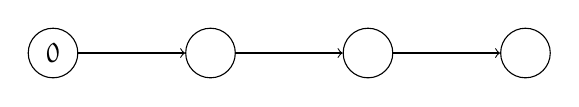
\begin{tikzpicture}
    \node (a) at (0,0) [circle, draw] {$0$}; \node (b) at (2,0)
    [circle,draw] {\phantom{$0$}}; \node (c) at (4,0) [circle,draw]
    {\phantom{$0$}}; \node (d) at (6,0) [circle,draw] {\phantom{$0$}};
    \draw[->] (a.east) -- (b.west); \draw[->] (b.east) -- (c.west);
    \draw[->] (c.east) -- (d.west);
  \end{tikzpicture}

\item
  
\begin{tikzpicture}
    \node (a) at (0,0) [circle, draw] {\phantom{$0$}};
    \node (b) at (2,0) [circle, draw] {\phantom{$0$}};
    \draw[->] (a.south east) .. controls (1,-.5) .. (b.south west);
    \draw[->] (b.north west) .. controls (1,.5) .. (a.north east);
  \end{tikzpicture}

\item  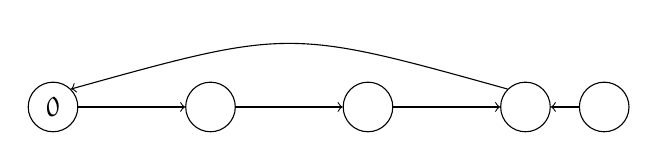
\begin{tikzpicture}
    \node (a) at (0,0) [circle, draw] {$0$}; \node (b) at (2,0)
    [circle,draw] {\phantom{$0$}}; \node (c) at (4,0) [circle,draw]
    {\phantom{$0$}}; \node (d) at (6,0) [circle,draw] {\phantom{$0$}};
    \node (e) at (7,0) [circle,draw] {\phantom{$0$}};
    \draw[->] (a.east) -- (b.west); \draw[->] (b.east) -- (c.west);
    \draw[->] (c.east) -- (d.west); \draw[->] (d.north west)
    .. controls (3,1) .. (a.north east);
    \draw[->] (e.west) -- (d.east);
  \end{tikzpicture}

\item
  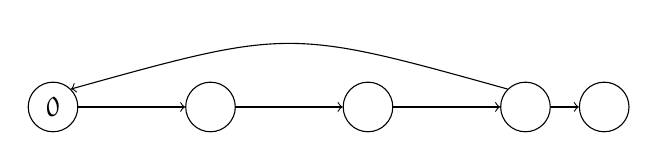
\begin{tikzpicture}
    \node (a) at (0,0) [circle, draw] {$0$}; \node (b) at (2,0)
    [circle,draw] {\phantom{$0$}}; \node (c) at (4,0) [circle,draw]
    {\phantom{$0$}}; \node (d) at (6,0) [circle,draw] {\phantom{$0$}};
    \node (e) at (7,0) [circle,draw] {\phantom{$0$}};
    \draw[->] (a.east) -- (b.west); \draw[->] (b.east) -- (c.west);
    \draw[->] (c.east) -- (d.west); \draw[->] (d.north west)
    .. controls (3,1) .. (a.north east);
    \draw[->] (d.east) -- (e.west);    
  \end{tikzpicture}

\end{enumerate}
\end{multicols}

\item\label{exer:cases} I have in mind a picture for Signature \ref{sig:Nat} and that satisfies Axioms \ref{ax:NatZero}
and \ref{ax:NatPred}. Furthermore, in that picture, I have in mind and element $n$ for which (a) $n\neq 0$
and (b) $n$ has no predecessor (that is, $n\neq m^\nxt$ for every $m$). Convince me that
the picture fails to satisfy Axiom \ref{ax:NatInd}.
%\end{itemize}
\end{exercises}

The latest exercise shows that in the natural numbers, if $n\neq 0$, then $n = m^\nxt$ for some $m$. In other
words, every non-zero natural number has a predecessor. 


\chapter{Arithmetic}

Adding and multiplying arise from counting. In this section, we explore how to define them purely in terms of counting.

\medskip
\begin{goals}
\tightlists
\noindent\textbf{Lecture}
\begin{itemize}
\item Present addition and multiplication via defining equations.
\item Practice using the defining equations to calculate sums and products.
\end{itemize}

\noindent\textbf{Study}
\begin{itemize}
  \item Understand addition and multiplication as characterized by defining equations.
  \item Be able to explain how addition and multiplication relate to counting.
  \item Exhibit competence in calculating sums and products from the defining equations.
\end{itemize}
\defaultlists
\end{goals}

\ipadbreak

\section{Basic Arithmetic Operations}

\begin{defn}\label{def:NatArithmetic}
\noindent The \emph{sum} of two natural numbers, $m$ and $n$, is a natural number (denoted by $m+n$). For every natural number $m$, the following 
are true:
\begin{align*}
    m + 0     &= m\\
    m + k^\nxt &= (m + k)^\nxt &&\text{for any natural number $k$}
\end{align*}

\noindent The \emph{product} of two natural numbers, $m$ and $n$, is a natural number 
(denoted by $m\cdot n$). For every natural number $m$, the following are true:
\begin{align*}
  m\cdot 0 &= 0\\
  m\cdot k^\nxt &= m + (m\cdot k) &&\text{for any natural number $k$}
\end{align*}
\end{defn}


A moment's thought about arithmetic should convince you that these equations are reasonable.
Certainly $m+0=m$ and $m\cdot 0 = 0$ should be true for any $m$. 
The second equation for $+$ can be read as saying ``to add $m$ to the successor of $k$,
simply add $m$ to $k$, then take the successor.'' The second equation for $\cdot$
can be read as saying ``to multiply $m$ by the successor of $k$, simply
multiply $m$ by $k$, and add $m$ to the result.''

But it is not the case that any arbitrary pair of equations involving $0$ and $k^\nxt$
will define anything sensible. In the cases of $+$ and $\cdot$, though, 
the Axiom of Induction ensures that there are indeed unique operations
that satisfy the equations. A proof of this fact is not particularly illuminating
right now, so let us agree to take for granted that the equations 
spelled out here actually define addition and multiplication.

\begin{example}
Do the defining equations for addition really explain how to add? Let's use them to calculate
$4+3$:
\begin{align*}
  4 + 3 &= 4 + 0^{\nxt\nxt\nxt}&&\text{[$3$ abbreviates $0^{\nxt\nxt\nxt}$]}\\
  &= 4^\nxt + 0^{\nxt\nxt} &&\text{[$m + k^\nxt = m^\nxt+k$]}\\
  &= 4^{\nxt\nxt} + 0^\nxt &&\text{[Same reason]}\\
  &= 4^{\nxt\nxt\nxt} + 0 &&\text{[Same reason]}\\
  &= 4^{\nxt\nxt\nxt} &&\text{[$m+0 = m$]}\\
  &= (0^{\nxt\nxt\nxt\nxt})^{\nxt\nxt\nxt} && \text{[$4$ abbreviates $0^{\nxt\nxt\nxt\nxt}$]}\\
  &= 0^{\nxt\nxt\nxt\nxt\nxt\nxt\nxt} && \text{[Remove unneeded parentheses]}\\
  &= 7 &&\text{[$7$ abbreviates $0^{\nxt\nxt\nxt\nxt\nxt\nxt\nxt}$]}
\end{align*}
\end{example}
\ipadbreak

\begin{example}
A product can be calculated similarly. Consider $2\cdot 2$.
\begin{align*}
  2\cdot 2 &= 2\cdot 0^{\nxt\nxt} &&\text{[$2$ abbreviates $0^{\nxt\nxt}$]}\\
           &= 2 + (2\cdot 0^\nxt) &&\text{[$m\cdot k^\nxt = m + (m\cdot k)$]}\\
           &= 2 + (2 + (2\cdot 0))&&\text{[Same reason]}\\
           &= 2 + (2 + 0) &&\text{[$m\cdot 0=0$]}\\
           &= 2 + 2&&\text{[$m+0 = m$]}\\
           &= 2 + 0^{\nxt\nxt}&&\text{[$2$ abbreviates $0^{\nxt\nxt}$]}\\
           &= 2^\nxt + 0^\nxt &&\text{[$m+k^\nxt = m^\nxt+k$]}\\
           &= 2^{\nxt\nxt} + 0&&\text{[Same reason]}\\
           &= 2^{\nxt\nxt} &&\text{[$m+0 = m$]}\\
           &= (0^{\nxt\nxt})^{\nxt\nxt} &&\text{[$2$ abbreviates $0^{\nxt\nxt}$]}\\
           &= 0^{\nxt\nxt\nxt\nxt}&&\text{[Remove unnecessary parentheses]}\\
           &= 4 &&\text{[$4$ abbreviates $0^{\nxt\nxt\nxt\nxt}$]}
\end{align*}
\end{example}

We certainly will not want to calculate this way in real life. 
After all, it took twelve steps just to figure $2\cdot 2=4$. But these
examples and the following exercises show how addition and multiplication are
closely tied to simple counting. 

\ipadbreak

\begin{exercises}
%\begin{itemize}
\item Calculate these sums, following the previous example to write
  each step of your calculation explicitly. Include the reason for
  each step (as in the previous example).Take care to lay out the
  chain of equalities correctly, and do not skip any steps.
\begin{enumerate}
\item $2+4$
\item $4+2$
\item $3+(3+1)$
\item $(3+3)+1$
\item $0 + 3$
\end{enumerate}

\item Notice that it takes more steps to calculate $2+4$ than $4+2$, even though we already knew
they would produce the same answer. Explain why.

\item Calculate the following values, writing each step explicity. 
 \begin{enumerate}
    \item $2\cdot 3$
    \item $0\cdot 2$
    \item $2\cdot(2\cdot 2)$
    \item $3\cdot(2 + 1)$
    \item $(3\cdot 2) + (3\cdot 1)$
    \end{enumerate}
\item Write a definition of exponentiation via defining equations. Follow the pattern
of definition I have written for addition and multiplication.
%\end{itemize}
\end{exercises}

\chapter{Laws of Arithmetic}

Before working the last exercises, you knew that $3\cdot (2+1)$ and $3\cdot 2+ 3\cdot 1$
would come out the same because of a law of arithmetic known as \emph{distributivity}. 
Addition and multiplication satisfy several other laws.

\begin{goals}
\noindent\textbf{Lecture}
\begin{itemize}
\item Present the most common Laws of Arithmetic for natural numbers.
\item Explain the method of \emph{proof by simple induction}
\item Prove a representative sample of the laws by simple induction.
\end{itemize}
\noindent\textbf{Study}
\begin{itemize}
\item Become familiar with the common names for the Laws of Arithmetic.
\item Pay particular attention to the Laws of Positivity and Cancellativity (they may be the least familiar to you).
\item Demonstrate the ability to identify the main parts of a proof by simple induction.
\item Demonstrate the ability to construct the parts of a proof by simple induction.
\item Prove the remaining laws for yourself.
\end{itemize}
\end{goals}

\ipadbreak

\section{Basic Laws}

The following list summarizes several useful laws of
arithmetic on the natural numbers. They are organized to emphasize
similarities between addition and multiplication.

\begin{laws}
\noindent For any natural numbers, $m$, $n$ and $p$:

\begin{tabular}{lr@{\,}l@{\qquad}lr@{\,}l}
\textbf{Associativity}& $m + (n + p)$      &$= (m+n)+p$           &\textbf{Commutativity}&$m + n$    &$= n + m$\\
                      &$m \cdot(n\cdot p)$ &$= (m\cdot n)\cdot p$ &                      &$m\cdot n$ &$= n\cdot m$\\
&&&&&\\ 
\textbf{Identity}&$m + 0$    &$= m$&\textbf{Positivity}&\multicolumn{2}{c}{if $m + n = 0$ then $m=0$}\\
                 &$m\cdot 1$ &$= m$&                   &\multicolumn{2}{c}{if $m\cdot n = 1$ then $m=1$}\\
&&&&&\\
\textbf{Cancellativity}&\multicolumn{2}{c}{if $m + p = n+p$ then $m=n$}&&&\\
                       &\multicolumn{2}{c}{if $m \cdot p^\nxt = n\cdot p^\nxt$ then $m=n$}&&&\\
&&&&&\\
\textbf{Distributivity}&$m\cdot(n+p)$&$= (m\cdot n) + (m\cdot p)$&&&\\
&&&&&\\
\textbf{Case Distinction}&\multicolumn{2}{c}{if $m\neq 0$ then $m=k^\nxt$ for some $k$}&&&\\
\end{tabular}
\end{laws}
\medskip

Most of these laws are familiar and are listed with their common names. The Law of Case
Distinction was the subject of Exercise \ref{exer:cases}. \emph{Go back and look at that exercise again}.
The Law of Positivity for multiplication is not a common name, but
I have used it to emphasize the analogies between addition and multiplication.
Also Case Distinction does not really have a common name. I made that up.

\ipadbreak

\section{Inductive Proofs}

Suppose we wish to prove that every natural number has some
property. For example, let us suppose we wish to prove that every
natural number is \emph{mimsy}.  I have no idea what a mimsy number
is, but let us try to prove this anyway. We could try proving that $0$
is mimsy, $1$ is mimsy, $2$ is mimsy, and so on.  But this won't work
because our proof will never end. In fact, it is not so obvious that
we, humans with finite minds, can ever prove that some property is
true for \emph{all} natural numbers, since it seems to involve
checking infinitely many individual cases.

The Axiom of Induction provides a way forward in spite of our
limitations.  Suppose we were to show that the mimsy natural numbers
all by themselves constitute a picture of Signature
\ref{sig:NatSig}.  Then there could not be any natural numbers
left out, for otherwise, we could erase all the non-mimsy natural
numbers and still have a picture of \ref{sig:Nat}. This
is exactly what the Axiom of Induction forbids: we can not erase
\emph{anything} without breaking the signature.

So to prove that all natural numbers are mimsy, we simply need to
prove that
\begin{itemize}
\item $0$ is mimsy, and
\item for all natural numbers $k$, if $k$ is mimsy so is $k^\nxt$.
\end{itemize}
From these, we conclude that the mimsy natural numbers by themselves form a picture of \ref{sig:Nat}. So the Axiom of Induction ensures that all natural numbers
are mimsy.

%\begin{usage}
%  A proof employing the Axiom of Induction in this way is called a
%  proof \emph{by simple arithmetic induction}, or just a proof \emph{by
%    induction}, for short.  We will see more general forms of
%  induction later.
%\end{usage}

To make inductive proofs easier to understand, we often write them
using a three step outline, as illustrated here.
\begin{itemize}
\item{}[Basis] Prove that $0$ is mimsy.
\item{}[Inductive Hypothesis] Assume that $k$ is mimsy.
\item{}[Inductive Step] Prove that $k^\nxt$ is mimsy. [You may use the
  assumption that $k$ is mimsy in this part of the proof.]
\end{itemize}

More practical examples are next.

\ipadbreak

\begin{fact}

  \emph{Addition is associative.}

\begin{proof}
  We need to show that $m + (n+p) = (m+n)+p$ for all $m$, $n$ and $p$.
  Let us suppose that $m$ and $n$ are fixed values (not known to us).
  We now prove that the values $p$ for which $m+(n+p) = (m+n)+p$ holds
  form a picture of \ref{sig:Nat}.
  \begin{itemize}
  \item{}[Basis] $m+(n+0) = m+n = (m+n)+0$. Both steps are due to the
    defining equations of $+$.
  \item{}[Inductive Hypothesis] Assume $m+(n+k) = (m+n)+k$.
  \item{}[Inductive Step] We must show that $m+(n+k^\nxt) =
    (m+n)+k^\nxt$. 
    \begin{align*}
      m+(n+k^\nxt) &= m + (n+k)^\nxt &&\text{[Def. of +]}\\
      &= (m+(n+k))^\nxt&&\text{[Same]}\\
      &= ((m+n)+k)^\nxt&&\text{[Inductive Hypothesis]}\\
      &= (m+n)+k^\nxt &&\text{[Def. of $+$]}
    \end{align*}
  \end{itemize}
  Therefore (by the Axiom of Induction), $m+(n+p) = (m+n)+p$ holds for
  all $p$. Since the argument does not depend on any extra assumptions
  about $m$ and $n$, it holds for all $m$ and $n$.
\end{proof}
\end{fact}

%\begin{usage}
  We say this proof is \emph{by induction on $p$} to emphasize that
  the variable $p$ is the focus of attention. The other variables are
  not directly involved in the structure of the proof.
%\end{usage}

The remainder of this section further illustrates the technique of
simple arithmetic induction via proofs of other laws of arithmetic.

\ipadbreak

\begin{fact}\label{lem:AddZero}
  $0$ is the identity for addition.

\begin{proof}
  We must prove that $m+0 = m = 0 + m$ for all $m$. The first equality is true by the definition of $+$.
  But the second equality, $m = 0 + m$, is not explicitly one of the defining facts about $+$. So we proceed by induction on $m$.
  \begin{itemize}
  \item{}[Basis] $0+0 = 0$ is true by definition of $+$.
  \item{}[Inductive Hypothesis] Assume $0 + k = k$.
  \item{}[Inductive Step] We must show that $0 + k^\nxt = k^\nxt$.
    \begin{align*}
      0 + k^\nxt &= (0+k)^\nxt &&\text{[Def. of $+$]}\\
      &= k^\nxt &&\text{[Inductive hypothesis]}
    \end{align*}
  \end{itemize}
  Therefore, $0+m=m$ holds for all $m$.
\end{proof}
\end{fact}

\ipadbreak

To prove that addition is commutative, we need an additional fact
about how successor and addition interact.

\begin{lemma}\label{lem:AddSucc}
  For any $m$ and $n$, $(m + n)^\nxt = m^\nxt + n$.

 \begin{proof}
   By induction on $n$:
   \begin{itemize}
   \item{}[Basis]
     \begin{align*}
       (m + 0)^\nxt &= m^\nxt     &&\text{[Def. of $+$]}\\
       &= m^\nxt + 0 &&\text{[Def. of $+$]}
     \end{align*}
   \item{}[Inductive Hypothesis]
    Assume $(m + k)^\nxt = m^\nxt + k$ for some $k$.
   \item{}[Inductive Step]
    We must show that $(m + k^\nxt)^\nxt = m^\nxt + k^\nxt$.
    \begin{align*}
      (m + k^\nxt)^\nxt &= ((m + k)^\nxt)^\nxt && \text{[Def. of $+$]}\\
                     &= (m^\nxt + k)^\nxt &&\text{[Inductive Hypothesis]}\\
                     &= m^\nxt + k^\nxt   &&\text{[Def. of $+$]}
    \end{align*}
   \end{itemize}
So $(m + n)^\nxt = m^\nxt + n$. Because the proof does not depend on any assumption about $m$, it is valid
for all $m$.
 \end{proof}
\end{lemma}

\ipadbreak

\begin{fact}

  \emph{Addition is commutative.}

\begin{proof}
  We need to show that $m+n = n + m$ for all $m$ and $n$.  This time,
  the proof is by induction on $m$. Fix a value for $n$.
  \begin{itemize}
  \item{}[Basis] $0 + n = n = n + 0$ holds because of Fact
    \ref{lem:AddZero} and the definition of $+$.
  \item{}[Inductive Hypothesis] Assume that $k + n = n + k$ for some
    $k$.
  \item{}[Inductive Step] We must show that $k^\nxt + n = n + k^\nxt$.
    \begin{align*}
      k^\nxt + n &= (k + n)^\nxt&&\text{[Lemma \ref{lem:AddSucc}]}\\
      &=  (n+k)^\nxt&&\text{[Inductive Hypothesis]}\\
      &= n + k^\nxt&&\text{[Def. of $+$]}
    \end{align*}
  \end{itemize}
  Therefore, $m + n = n + m$ for all $m$. Since this argument does not
  depend on any assumptions about $n$, it is valid for all $n$.
\end{proof}
\end{fact}
\ipadbreak

\begin{fact}
  \emph{Addition is cancellative.}

\begin{proof}
  We need to prove that if $m + p= n+p$, then $m=n$.  This proof is a little subtler than the previous ones. But notice that is
  still follows the same form.
  
  The proof is by induction on $p$. Assume that $m$ and $n$ are some fixed natural numbers.
  \begin{itemize}
  \item{}[Basis] Suppose $m+0 = n+ 0$. Then immediately by definition
    of $+$, $m=n$.
  \item{}[Inductive Hypothesis] Assume that the following statement is true for some $k$: if $m + k = n + k$ then $m=n$.
  \item{}[Inductive Step] We must show that 
    if $m+k^\nxt = n+k^\nxt$ then $m=n$. Suppose $m+k^\nxt = n + k^\nxt$ [call this (*) for reference]. Then
    \begin{align*}
      (m+k)^\nxt & = m + k^\nxt &&\text{[Def. of $+$]}\\
      & = n + k^\nxt &&\text{[By the supposition (*)]}\\
      & = (n+k)^\nxt &&\text{[Definition of $+$]}
    \end{align*}
    Hence, by Axiom \ref{ax:NatPred} $m+k=n+k$. So by the Inductive Hypothesis, $m=n$.
  \end{itemize}
  Therefore, $m + p = n + p$ implies $m = n$ for all $p$. Since this argument does not
depend on any assumptions regarding $m$ and $n$, it is valid for all $m$ and $n$.
\end{proof}
\end{fact}
\ipadbreak

To prove that multiplication is commutative and cancellative, we will
need the following technical facts (analogous to Lemmas
\ref{lem:AddZero} and \ref{lem:AddSucc}).

\begin{lemma}\label{lem:MultZero}
  $0\cdot n = 0$

  \begin{proof}
    The proof is by induction on $n$.
    \begin{itemize}
    \item{}[Basis] $0\cdot 0 = 0$ by definition of $\cdot$.
    \item{}[Inductive Hypothesis] Assume that $0\cdot k = 0$ for some
      $k$.
    \item{}[Inductive Step] We must show that $0\cdot k^\nxt = 0$.
      \begin{align*}
        0\cdot k^\nxt &= 0 + 0\cdot k &&\text{[Definition of $\cdot$]}\\
        &= 0 + 0 &&\text{[Inductive Hypothesis]}\\
        &= 0&&\text{[Definition of $+$]}
      \end{align*}
    \end{itemize}
  \end{proof}
\end{lemma}

\ipadbreak

\begin{lemma}\label{lem:MultSucc}
  $m^\nxt \cdot n = m\cdot n + n$

 \begin{proof}
   The proof is by induction on $n$.
   \begin{itemize}
   \item{}[Basis] $m^\nxt\cdot 0 = 0 = 0+0 = m\cdot 0 + 0$ all follow
     from the definitions of $+$ and $\cdot$.
   \item{}[Inductive Hypothesis] Assume that $m^\nxt\cdot k = m\cdot k +
     k$ for some $k$.
   \item{}[Inductive Step] We must show that $m^\nxt\cdot k^\nxt =
     m\cdot k^\nxt + k^\nxt$.
     \begin{align*}
       m^\nxt\cdot k^\nxt &= m^\nxt + m^\nxt\cdot k &&\text{[Def. of $\cdot$]}\\
       &= (m + m^\nxt\cdot k)^\nxt &&\text{[Lemma \ref{lem:AddSucc}]}\\
       &= (m + (m\cdot k + k))^\nxt && \text{[Inductive Hypothesis]}\\
       &= ((m+ m\cdot k) + k)^\nxt &&\text{[Associativity of $+$]}\\
       &= (m\cdot k^\nxt + k)^\nxt &&\text{[Def. of $\cdot$]}\\
       &= m\cdot k^\nxt + k^\nxt &&\text{[Def. of $+$]}
     \end{align*}
   \end{itemize}
 \end{proof}
\end{lemma}

Other laws are left as exercises.

\ipadbreak

\begin{exercises}
  % \begin{enumerate}
\item Prove that $1$ is the identity for multiplication. That is $1\cdot m = m  = m\cdot 1$.
\item Prove that multiplication distributes over addition [$m\cdot
  (n+p) = m\cdot n + m\cdot p$] by induction on $p$.  You can use the
  fact that addition is associative and commutative because we have
  already proved those.
  \begin{enumerate}
  \item Prove the basis: $m\cdot(n+0) = m\cdot n + m\cdot 0$.
  \item Write the inductive hypothesis.
  \item Prove the inductive step: $m\cdot(n+k^\nxt) = m\cdot n +
    m\cdot k^\nxt$
  \end{enumerate}
 
\item Prove that multiplication is associative [$m\cdot(n\cdot p) =
  (m\cdot n)\cdot p$] by induction on $p$.
  \begin{enumerate}
  \item Prove the basis: $m\cdot (n\cdot 0) = (m\cdot n)\cdot 0$.
  \item Write the inductive hypothesis.
  \item Prove the Inductive Step: $m\cdot (n\cdot k^\nxt) = (m\cdot
    n)\cdot k^\nxt$. Hint: Use the Law of Distribution, which you just
    proved.
  \end{enumerate}

\item Prove that multiplication is commutative. Hint: Use the two facts 
we proved riht before these exercises.

  % \end{enumerate}
\end{exercises}

\ipadbreak

For the record, we also prove the cancellation law for multiplication. This is 
a bit harder than the exercises, but you should try to find your own proof before looking at mine.

\begin{fact}

  \emph{If $m\cdot p^\nxt = n\cdot p^\nxt$, then $m=n$.}

\begin{proof}
  The proof is by induction on $n$.
  \begin{itemize}
  \item{}[Basis] Suppose $m\cdot p^\nxt = 0\cdot p^\nxt$. From Fact
    \ref{lem:MultZero}, $m+ m\cdot p = m\cdot p^\nxt = 0$. So the Law of
    Positivity for addition ensures that $m=0$.
  \item{}[Inductive Hypothesis] Assume that for some $k$, the following is true:
    if $m\cdot p^\nxt = k\cdot p^\nxt$, then $m=k$.
  \item{}[Inductive Step] Suppose that $m\cdot p^\nxt = k^\nxt \cdot
    p^\nxt$. Then
    \begin{align*}
      m\cdot p^\nxt &= k^\nxt\cdot p^\nxt &&\text{[By assumption]}\\
      &= k\cdot p^\nxt + p^\nxt &&\text{[Lemma \ref{lem:MultSucc}]}\\
      &= (k\cdot p^\nxt + p)^\nxt &&\text{[Definition of $+$]}\\
      &\neq 0 &&\text{[Axiom Nat \ref{ax:NatZero}]}
    \end{align*}
    Consequently, $m\neq 0$, for otherwise we would have $m\cdot
    p^\nxt = 0$. Since $m$ is not equal to $0$, it is equal to some
    successor (by the Case Distinction Law). Let $j$ be the predecessor of $m$,
	so that $j^\nxt=m$.
    \begin{align*}
      j\cdot p^\nxt + p^\nxt & m\cdot p^\nxt &&\text{[Lemma \ref{lem:MultSucc}]}\\
      &= k^\nxt \cdot p^\nxt &&\text{[By supposition]}\\
      &= k\cdot p^\nxt + p^\nxt &&\text{[Lemma \ref{lem:MultSucc}]}
    \end{align*}
    Because addition is cancellative, $j\cdot p^\nxt = k\cdot
    p^\nxt$. Now, the Inductive Hypothesis ensures that $j=k$. Hence
    $m = j^\nxt = k^\nxt$.
  \end{itemize}
\end{proof}
\end{fact}

%%% Local Variables: 
%%% mode: latex
%%% TeX-master: "MainText"
%%% End: 


% 1
%\input{ListsStructures.tex}
%\chapter{Other Number Systems}\label{lec:OtherNumbers}

Discrete Mathematics is not only concerned with natural numbers. Integers, rational numbers, real numbers and even, on a few occasions, complex numbers, all play their roles. In this lecture, we discuss, with much less formality, integers and rational numbers, leaving real and complex numbers to a courses on analysis.

\begin{goals}
\begin{goal}{Lecture}
\item Introduce the standard notation for these number systems.
\item Discuss briefly the extensions of arithmetic to integers, rationals.
\item Wave hands and mumble unconvincingly about real and complex numbers.
\end{goal}

\begin{goal}{Study}
\item Learn the meanings of the symbols for standard number systems.
\item Prove some simple facts about arithmetic on integers and rational numbers.
\end{goal}
\end{goals}

\section{Integers}

Our intention here is to give a general overview of the integers in light of our detailed study of natural numbers.
Though we could, we will not go into the same level of detail.

Integers, we understand, include the natural numbers but also include negatives. They constitute the simplest possible extension of the natural numbers in such a way so that for any integers $a$ and $b$, there is a solution of the equation $a = b + x$.  
So the fundamental structure of integers is that (a) the natural numbers are integers and (b) addition on integers is invertible, i.e., subtraction works correctly.

\begin{postulate}\label{post:IntSignature}
The integers have the following basic structure.

\begin{itemize}
\item Every natural number is an integer. For this discussion, we will use letters $a$, $b$, $c$, \ldots for integers,
and $m$, $n$, \ldots for natural numbers.
To emphasize when a natural number $m$ plays the role of an integer we write ${}^+m$.
\item For every two integers, $a$ and $b$, there is a \emph{sum} and a \emph{difference}, denoted by $a+b$ and $a-b$. 
\end{itemize}
\end{postulate}

We must insist that addition on integers behaves as we should expect. 
\begin{postulate}\label{post:IntAddition}
For natural numbers $m$ and $n$,
\[{}^+m + {}^+n = {}^+(m+n).\]
That is, adding $m$ and $n$ \emph{as integers} is the same as adding them \emph{as natural numbers}.

Furthermore, addition on integers is associative and commutative, and $a + {}^+0 = a$ for all integers $a$.
\end{postulate}

Next, sum and difference are related.

\begin{postulate}\label{post:IntSubtraction}
For any integers $a$, $b$ and $c$, 
\[a = b + c\quad\text{if and only if}\quad a - b = c\]
\end{postulate}

Finally, we require minimality.

\begin{postulate}\label{post:IntInduction}
  No integers can be removed without violating Postulate \ref{post:IntSignature}.
\end{postulate}

We do not go through the details, but these axioms determine the structure of the integers similar to the way our earlier axioms determine the structure of the natural numbers. 
Moreover, all the familiar laws of addition and subtraction follow.
We illustrate with two simple laws. 
As usual, we can abbreviate ${}^+0-a$ by $-a$.

\begin{lem}\label{lem:IntAdditiveInverse}
For any integer $a$, ${}^+0= a + -a$.

\begin{proof}
  Since ${}^+0-a = {}^+0-a$ (trivially), Postulate \ref{post:IntSubtraction} yields ${}^+0 = a + ({}^+0-a) = a + (-a)$.
\end{proof}
\end{lem}

\begin{lem}\label{lem:IntAddSub}
  For integers $a$ and $b$, $a-b = a + (-b)$.

  \begin{proof}
    $a = a + {}^+0 = a + (-b + b) = b + (a+(-b))$ by the basic laws of addition (identity, commutativity and associativity)
and the previous lemma. So by Postulate \ref{post:IntSubtraction}, $a-b = a + (-b)$.
  \end{proof}
\end{lem}

In the axiomatization of integers, we did not mention multiplication. This is because multiplication is definable from addition. But we need an aditional fact.

Say that an integer $a$ is ``simple'' if either $a={}^+m$ or $-a = {}^+m$ for some natural number $m$. 

\begin{lem}
	Every integer is simple.
	
	\begin{proof}
		Exercise
	\end{proof}
\end{lem}

\begin{defn}
For any two integers $a$ and $b$, the \emph{product} $a\cdot b$ defined as follows:
\begin{align*}
	a\cdot {}^+0 &= {}^+0\\
	a\cdot {}^+(k^\nxt) &= a + a\cdot {}^+k\\
	a\cdot -({}^+m) &= -(a\cdot {}^+m)
\end{align*}
\end{defn}

These requirements are enough to ensure that multiplication is the operation we expect it to be.
We will not verify that fact, but it involves an inductive argument similar to the arguments that we saw in previous lectures.

\begin{exer}
	\begin{exercise}
\item Show that every integer is simple, using only the postulates given here.

Hint: First observe that, trivially, every integer of the form ${}^+m$ is simple.
This acts as the basis for an inductive proof. 
Now suppose $a$ and $b$ are simple (the inductive hypothesis).
Show that both $a+b$ and $a-b$ are simple (the inductive step).
Since the integers are minimal for including the natural numbers and being closed under $+$ and $-$, this shows that all integers are simple.
\item Using only the axioms for integers, the foregoing two lemmas and the definition of multiplication, prove the following (remember
that $-a$ abbreviates ${}^+0 - a$). 
You should prove these in the order presented here, as later exercises may depend on earlier ones. For all integers $a$, $b$ and $c$ show that the following are true.
\begin{enumerate}
\item Addition is cancellative: $a + c = b + c$ implies $a = b$.
\item $a-b = -(b-a)$
\item $(a+b) - c = a + (b-c)$
\item $a-(b+c) = (a-b)-c$
\item $-(-a) = a$
\item ${}^+0\cdot a = {}^+0$
\item $-a\cdot -b = a\cdot b$
\item Multiplication distributes over addition.
\end{enumerate}
\end{exercise}
\end{exer}

\section{Rational Numbers}

Rational numbers, roughly, are minimal with respect to the integers and inverting multiplication, as 
integers are minimal with respect to natural numbers and inverting addition. Care must be taken, however, because ${}^+0\cdot a = {}^+0\cdot b$ is always true, this does not tell us anything about $a$ and $b$. So ``division by $0$'' can not make sense.  

\begin{postulate}\label{post:RatSignature}
The rational numbers have the following basic structure.
\begin{itemize}
\item Every integer is a rational number. For this discussion, to emphasize when an integer $a$ plays the
role of a rational number, we write $\frac{a}{1}$. 
\item For every two rational numbers $p$ and $q$, there is a \emph{product}, denoted by $p\cdot q$.
Moreover, if $q\neq \frac{0}{1}$, then there is a \emph{quotient}, denoted by $p/q$.
\end{itemize}
\end{postulate}

In analogy with integers, where addition and subtraction are the main operations, we insist that
multiplication behaves correctly. 

\begin{postulate}\label{post:RatMultiplication}
For integers $a$ and $b$,
\[\frac{a}1 \cdot \frac{b}1 = \frac{ab}1\]
That is, multiplying integers $a$ and $b$ \emph{as rational numbers} is the same as multiplying them \emph{as integers}.

Furthermore, multiplication is associative and commutative, and $p \cdot \frac{1}{1} = p$ for all rational numbers $p$.
\end{postulate}

Again, continuing the analogy with integers, multiplication and division must cooperate.
\begin{postulate}\label{post:rationaldivision}
For any rationals $p$, $q$ and $r$,
if $q\neq \frac{0}1$, then 
\[p= q \cdot r\quad\text{if and only if}\quad p/q = r\]
\end{postulate}

Finally, we require minimality.

\begin{postulate}\label{post:RationalInduction}
  No rational numbers can be removed without violating Postulate \ref{post:RatSignature}.
\end{postulate}

Like the axioms for integers, these axioms completely determine the rational numbers along with multiplication and division. 
To extend addition and subtraction to the rational numbers we can require the following.

For integers, we introduced the idea of \emph{simplicity} to capture the fact that every integer is either a natural number or a negated natural number. The analogous idea for rational numbers is that every rational number is expressible as a fraction.

\begin{defn}
	Say that a rational number $p$ is \newterm{fractional} if it is the case that $p=a/b$ for some integer $a$ and non-zero integer $b$. 
\end{defn}

\begin{lem}
	Every rational number is fractional.
	
	\begin{proof}
		Like the proof that every integer is simple, this involves an inductive argument. Namely, every integer is, according to the basic structure of rationals, fractional. Namely, $a/{}+1 = \frac{a}1$. Indeed the difference between the two notations is almost trivial.
		For the sake of completeness though, note that an integer $a$ is written as $\frac{a}{1}$ only to emphasize that it is also a rational number. So $a/{}^+1 = a$ because $a = {}^+1\cdot a$.
		
		Suppose $p$ and $q$ are fractional. So $p=a/b$ and $q=c/d$ for some integers $a$, $b$, $c$ and $d$ with $b\neq 0$ and $d\neq 0$. Note that $a/b = p$ means that $a=b\cdot p$. Likewise $c=d\cdot q$. We claim that $p\cdot q = (a\cdot c)/(b\cdot d)$. This is true if
		$p\cdot q \cdot b\cdot d = a\cdot c$. But this follows from the foregoing. Since $b$ and $d$ are not zer, $b\cdot d$ is not zero. Hence $p\cdot q$ is fractional.
		We also claim that $p/q$ is fractional. Here we need two cases. Suppose $c=0$. Then $p=0/1$ as needed. Suppose $c\neq 0$. 
		Then $p/q = (a\cdot d)/(b\cdot c)$ because $a\cdot d \cdot q = p b\cdot c\cdot p$. We leave it to the reader to figure out why this last equation is true.
	\end{proof}
\end{lem}

Notice that this lemma does not tell us anything about simplified fractions. It merely says that every rational number can be written as a fraction. But over course, $2/4 = 4/8 = 6/12$ and so on.

\begin{defn}
For any two rational numbers $p = a/b $ and $q=c/d$, their \emph{sum}, denoted by $p+q$ is the rational number $(ad+cb)/bd$.
\end{defn}

This definition is not entirely legitimate yet. Because it could be the case that the result $(ad+cb)/bd$ depends on how we write $p$ and $q$ as fractions. In fact, though, this is not the case. For suppose $a/b = a'/b'$
and $c/d=c'/d'$. Then $(ad+cb)/bd = (a'd'+c'b')/b'd'$. So the way we add \emph{fractions} is correct for adding rational numbers.
These requirements are enough to ensure that addition is the operation we expect it to be. 

Now suppose $a$ is an integer and $m$ is a positive natural number. Then we
can write $\frac{a}m$ as an abbreviation of $\frac{a}{1} / \frac{{}^+m}1$. This is
the usual \emph{fraction} notation for rational numbers.
For a non-zero rational number $p$, we also usually write $p^{-1}$ to abbreviate 
$\frac{{}^+1}{1}/ p$.

\begin{exer}
\begin{exercise}
\item Using the proof of Lemma \ref{lem:IntAdditiveInverse} as a prototype, show that if $p\neq 0$,
then $p\cdot p^{-1} = 1$. 
\item Using the proof of Lemma \ref{lem:IntAddSub} as a prototype, show that if $q\neq \frac{{}^+0}{1}$ then $p/ q = p\cdot q^{-1}$.
\item Just using our axioms and the fraction notation (and the previous two exercises),
show that $\frac{4}{6} = \frac{2}{3}$.
\end{exercise}
\end{exer}

\section{Real and Complex Numbers}

We will not deal with rigorous characterizations of the real numbers and complex numbers in this course. 
A first course in real analysis is the appropriate place for such considerations. 
We simply take for granted that $\RR$ constitutes a suitable
extension of $\QQ$ to account for \emph{limits} (the mathematics you know from calculus). Likewise, $\CC$
constitutes a suitable extension of $\RR$ to account for 
algebraic closure (all polynomials having roots). The main things to know are that every rational number is real,
every real number is complex, and arithmetic operations behave as they should for real and complex numbers.

\begin{exer}
\begin{exercise}
  \item Relax. Take a walk.
\end{exercise}
\end{exer}

% 1
%\input{PythonPrimer.tex}
%\input{SumAndProduct.tex}

% 1
%\input{Numerals.tex}

% 2
%\chapter{Ordering the Natural Numbers by Addition}\label{lec:NatOrdering}

We have used the ordering of numbers informally without much comment
because $\leq$ has its obvious meaning. In this lecture 
we exploit the fact that $\leq$ on the natural numbers is defined by addition, setting the stage for an
analogous concept defined by multiplication. The multiplicative
analogue of ``$m$ is less than or equal $n$'' is ``$m$ divides $n$''.

\begin{goals}
\begin{goal}{Lecture}
\item Introduce a formal definition of $\leq$ on natural numbers, and discuss simple facts about order
%\item Introduce formal definitions $\min$ and $\max$ as dual concepts
\item Review basic laws involving $\min$ and $\max$.
\item Introduce Strong Induction and the Principle of Well-foundedness as alternatives to Simple Induction.
\end{goal}

\begin{goal}{Study}
\item Prove basic facts about $\leq$, $\min$ and $\max$.
\item Commit to memory the concepts of reflexivity, transitivity, anti-symmetry and linearity.
\item Practice using Strong Induction.
\end{goal}
\end{goals}


\section{Less or Equal}

For the natural numbers, $\leq$ has a particularly simple definition.

\begin{defn}
  For natural numbers $n$ and $m$, say that \emph{$m$ is less than or equal to $n$} (written $m\leq n$)
  if and only if there is a
  natural number $d$ so that $m+d = n$.  [I've used the letter $d$
  because $d$ is the \emph{difference} of $m$ from $n$.]
  
  Also, say that \newterm{$m$ is (strictly) less than $n$} if and only if there is a natural number $d$ so that $m + d^\nxt = n$.
\end{defn}

All of the usual properties of $\leq$ for natural numbers follow
easily from this definition using only the laws of
addition. The important properties have names.

\begin{laws} 
\begin{description}
	\item[Reflexivity] $\leq$ is \emph{reflexive}: $m\leq
m$ is true for any $m$. This is simply because because $m + 0 =
m$. 
    \item[Transitivity] $\leq$ is \emph{transitive}: if $m\leq
n$ and $n\leq p$, then $m\leq p$. Transitivity follows from the law of
associativity for addition (you will prove this as an exercise).
    \item[Anti-symmetry] $\leq$ is \emph{anti-symmetric}: if $m\leq n$ and $n\leq m$, then
	$m=n$. This follows from cancellativity and positivity (another exercise).
	\item[Linearity] $\leq$ is \emph{linear}: for any $m$ and $n$, either $m\leq n$ or $n\leq m$. This requires a separate proof using induction, dealt with below.
\end{description}
\end{laws} 

Clearly, $\leq$ is also meaningful for integers, rational numbers and real numbers, and is still reflexive, transitive and anti-symmetric and linear for them.
For our purposes, though, the interesting features are already present in the natural numbers.
For one thing, if $m+d = n$ and $m+e = n$ then $d=e$ (why?). This tells us that $m\leq n$ can only be true for one reason.

\ipadbreak

\begin{exer}
	In the following you will use the Laws of Arithmetic from Lecture \ref{lec:ArithmeticLaws} to prove the basic facts about $\leq$.
	\begin{exercise} 
    \item Show that $\leq$ is transitive by the following steps.
    \begin{enumerate}
    \item Assume that $m\leq n$. By definition, there is some $d_0$ so
      that $m+d_0 = n$
    \item Assume that $n\leq p$. Write out what this means. ``By
      definition, there is some \ldots''
    \item Now find an $e$ so that $m+e = p$.
    \item Write out the conclusion.
    \end{enumerate}

    \item Show that $\leq$ is anti-symmetric by the following steps.
    \begin{enumerate}
    \item Assume $m\leq n$. Write out what this means: ``There is some
      $d_0$ so that \ldots.''
    \item Assume $n\leq m$. Write out what this means. ``There is some
      $d_1$ so that \ldots.''
    \item Show that $d_0 + d_1 = 0$. [Think about using
      cancellativity.]
    \item Conclude that $d_0 = 0$. [Which law justifies this?]
    \item Conclude that $m = n$.
    \end{enumerate}
	\end{exercise}
\end{exer}

As we mentioned, $\leq$ is \emph{linear}, meaning
that for any $m$ and $n$, either $m\leq n$ or $n\leq m$. A proof of
this is not terribly difficult, but is more subtle than transitivity and anti-symmetry.

\begin{lem}
  \emph{$\leq$ is linear.}

  \begin{proof}
  	Note that we defined linearity in terms of $\leq$, but it is equivalent to saying that for any $m$ and $n$, either $m<n$ )or $n\leq m$. After all, if $m<n$ then $m\leq n$. And if $m\leq n$, then either $m=n$ and hence $n\leq n$, or $m<n$.  
    A proof is by induction on $m$.
    \begin{itemize}
    \item{}[Basis] $0 + n = n$ is always true. So $0\leq n$.
    \item{}[Inductive Hypothesis] Suppose that for some $k$, it
      is the case that either
      $k\leq n$ or $n\leq k$ (but we do not know which comparison is true).
    \item{}[Inductive Step] We must show that either $k^\nxt \leq n$ or
      $n\leq k^\nxt$.  According to the Inductive Hypothesis, there
      are two cases to consider. Either $k\leq n$ or $n\leq k$. We take them in reverse.
      \begin{enumerate}
      	\item Suppose $n\leq k$. 
	      	Then obviously $n\leq k^\nxt$ (meaning, it is so obvious that we do not bother to fill in the details).
		    \item Suppose $k< n$. So for some $d$, $k+d^\nxt =n$. Hence $k^\nxt+d=n$. if $d=0$, then $k^nxt = n$, so $n\leq k^\nxt$. Otherwise, $k^\nxt < n$.
      \end{enumerate}
    \end{itemize}
  \end{proof}
\end{lem}

\begin{exer}
	The following proofs should require you only to refer to the definition of $\leq$ and to the basic Laws of Arithmetic.
	\begin{exercise}
		\item Prove that addition is \newterm{monotonic} with respect to $\leq$. This means that $m\leq n$ implies $m+p\leq n+p$ for all natural numbers $m$, $n$ and $p$.
		\item Prove that addition is \newterm{order reflectiing} with respect to $\leq$. This means that if $m+p\leq n+p$, then $m\leq n$.
	\end{exercise}
\end{exer}

\section{Other Forms of Induction}

Using $\leq$, we can formulate a more flexible method of proof by induction.

Suppose we wish to prove that all natural numbers are \emph{outgrabe}.
Again this is nonsense, but let's try anyway. We prove the basis with no trouble; formulate the Inductive Hypothesis; get stuck on the Inductive Step.
Here is a simple idea that can help. 
Define a \emph{hypergrabe} number to be a natural number $k$ so that for every $j<k$, $j$ is outgrabe.
In other words, $k$ does not necessarily have the property we really care about, but all the numbers below it do.
Now suppose every natural number is outgrabe.
Then clearly, every natural number is also hypergrabe.
Likewise, if every natural number is hypergrabe, then every natural number is outgrabe.
So proving either property by induction will suffice to prove the other.
A proof by simple induction that all natural numbers are hypergrabe amounts to this:
\begin{itemize}
	\item{}[Basis] Show that every natural number $j<0$ is outgrabe. But since there are no such numbers, this is trivially true no matter what outgrabe happens to mean.
	\item{}[Inductive Hypothesis] Suppose that $k$ is hypergrabe for some $k$.
	That is, suppose that for all $j<k$, $j$ is outgrabe.
	\item{}[Inductive Step] Prove that $k^\nxt$ is hypergrabe.
	By the Inductive Hypothesis, all $j<k$ are outgrabe.
	So to prove that every $j<k^\nxt$ is outgrabe just amounts to
  proving it for $k$.
  So the Inductive Step (for proving that $k^\nxt$ is hypergrabe) amounts to proving that $k$ is outgrabe. 
\end{itemize}

This can now be reformulated without mentioning \emph{hypergrabe} at
all.  
The Basis is not needed, because it is true automatically.  
The Inductive Hypothesis can be reformulated as supposing that for all $j<k$, $j$ is outgrabe. 
The proof of the Inductive Step amounts to proving that $k$ is outgrabe.

This leads to a formulation of induction that is typically called
\emph{Strong Induction}, even though it is not really any stronger (i.e., it is not able to prove more facts).
A proof of property $P$ by Strong Induction has the outline:
\begin{itemize}
\item{}[Strong Inductive Hypothesis] Suppose that $P(j)$ is true for all $j<k$.
\item{}[Strong Inductive Step] Prove that $P(k)$ is true.
\end{itemize}

Exercises involving strong inductive proofs are not easy to come by right now.
We will see a very important example when we prove that every positive natural number can be factored into primes.

\begin{example}
Here is an example that uses strong induction to prove something. Define Fibonnacci number $f_n$ by the equations
\begin{align*}
  f_0 &= 0\\
  f_1 &= 1\\
  f_{n+2} &= f_{n+1} + f_n & \text{for any $n$}
\end{align*}
We claim that for all $n$, $2f_n \leq f_{n+2}$.

\begin{itemize}
\item{}[Strong Inductive Hypothesis] Suppose that for all $j<k$, $2f_j \leq f_{j+2}$.
\item{}[Strong Inductive Step]. We need to show that the claim also holds 
for $k$.
In case $k=0$, this is obviously true because $2f_0 = 0$. In case
$k=1$, it is also obviously true because $2f_1 = 2 = f_3$. 
In all other cases $k=i+2$ for some $i$. So 
\begin{align*}
2f_k  &= 2f_i + 2f_{i+1}&&\text{[By definition of $f$ and distributivity]}\\ 
      &\leq f_{i+2} + f_{i+3}&&\text{[By Inductive Hypothesis]}\\
      &= f_k + f_{k+1}&&\text{[$i+2=k$]}\\
      &= f_{k+2}&&\text{[By definition of $f$]}
    \end{align*}
\end{itemize}
\end{example}

We close this section with another method for using induction that is sometimes useful. 

\begin{lemma}\label{lem:N-well-ordered}
Suppose $P(-)$ is a property that makes sense for natural numbers. Suppose, furthermore, that $P(m)$ is
true for some $m$. Then there is a smallest $m$ for which $P(m)$ is true. That is, there is
a natural number $m_0$ so that $P(m_0)$ and so that $P(n)$ implies $m_0\leq n$. 
\begin{proof}
  Suppose $P(-)$ is a property that makes sense for natural numbers and that there is no
minimal $m$ for which $P(m)$ is true. We will show that $P(m)$ is false for all $m$ by strong induction.
\begin{itemize}
\item{}[Strong Inductive Hypothesis] Assume that $P(j)$ is false for all $j<k$.
\item{}[Inductive Step] We must show that $P(k)$ is also false. Suppose $P(k)$
were true. By the strong inductive hypothesis, $P(j)$ is false for all $j<k$. So $k$ would be the smallest
natural number for which $P(k)$ is true. This contradicts the assumption that there is no minimal value
for which $P(m)$ is true. So $P(k)$ must not be true.
\end{itemize}
\end{proof}
\end{lemma}

\begin{exer}
	\begin{exercise}
		\item Define the ``tribonacci'' numbers as follows:
		\begin{align*}
			t_0 &= 0\\
			t_1 &= 1\\
			t_2 &= 2\\
			t_{n+3}& = t_{n+2} + t_{n+1} + t_n & \text{for each $n$} 
		\end{align*}
		Prove by strong induction that $t_n < 2^{n-1}$ is true for all natural numbers $n$. [Recall that $2^{-1} = \frac{1}{2}$.]
		\item Prove that $n^3<3^n$ for all natural numbers $n$.
	\end{exercise}
\end{exer}

\section{Minimum and Maximum}

The minimum of two numbers $m$ and $n$ is, of course, the smaller of the two. 
We write $\min(m,n)$ for this. The maximum is written as $\max(m,n)$. To make this
precise, we can write a formal definition.

\begin{defn}
  For natural numbers $m$ and $n$, $\min(m,n)$ is a natural number satisfying:
  \begin{itemize}
  \item $\min(m,n)\leq m$ and $\min(m,n)\leq n$;
  \item for any natural number $p$, if $p\leq m$ and $p\leq n$, then $p\leq \min(m,n)$.
  \end{itemize}

Also, $\max(m,n)$ is defined \emph{dually}. For natural numbers $m$ and $n$, $\max(m,n)$ is a natural number satisfying:
\begin{itemize}
	\item $m\leq \max(m,n)$ and $n\leq \max(m,n)$;
	\item for any natural number $p$, if $m\leq p$ and $n\leq p$, then $\max(m,n)\leq p$.
\end{itemize}
\end{defn}


Both $\min$ and $\max$ are characterized by what we may call an ``adjoint situation''.
\begin{align*}
  p\leq \min(m,n) &\iff \text{$p\leq m$ and $p\leq n$}\\
  \max(m,n) \leq p&\iff \text{$m\leq p$ and $n\leq p$}
\end{align*}
This shows that comparing $p$ to two numbers on the right is the same as comparing $p$ to their minimum on the right; and similarly for comparison on the left and maximum.
We say that $\min(m,n)$ is the \emph{greatest lower bound} of $m$ and $n$ and that $\max(m,n)$ is the \emph{least upper bound} of $m$ and $n$. 

Some simple facts about $\min$ and $\max$ derive directly from this characterization by adjointness.
The two operations, $\min$ and $\max$, have many useful properties,
all of which can be proved using the above characterizations plus some facts about addition.

In particular, together with addition,  $\min$ and $\max$ make the natural numbers into something called a \emph{distributive lattice ordered monoid}.
Basically, this means that addition together with $\min$ and $\max$ cooperate in specific ways that are akin to the basic laws of arithmetic.
The most useful laws having to do with $\min$ and $\max$ are:


\begin{laws}[$\min$ and $\max$]\label{laws:minmax}
For all natural numbers $m$, $n$ and $p$:
	\begin{description} 
\item[Commutativity]
  \begin{align*}
    \min(m,n) &= \min(n,m)
    & \max(m,n) &= \max(n,m)\\
  \end{align*}
\item[Associativity]
  \begin{align*}
    \min(\min(m,n),p) &= \min(m,\min(n,p)) & \max(\max(m,n),p) &=
    \max(m,\max(n,p))
  \end{align*}
\item[Idempotency]
  \begin{align*}
    \min(m,m) &= m & \max(m,m) = m\\
  \end{align*}
\item[Absorption]
  \begin{align*}
    \min(m,\max(n,m)) &= m &\max(m,\min(n,m)) &= m
  \end{align*}
\item[Distributivity]
  \begin{align*}
    m + \min(n,p) &= \min(m+n,m+p) & m + \max(n,p) &= \max(m+n,m+p)\\
    \max(m,\min(n,p)) &= \min(\max(m,n),\max(m,p)) & \min(m,\max(n,p)
    &= \max(\min(m,n),\min(m,p))
  \end{align*}
\item[Modularity]
  \begin{align*}
    m + n &= \min(m,n) + \max(m,n)
  \end{align*}
  \end{description}
\end{laws}

We will not prove most of these as they follow easily from arithmetic laws. But the most subtle is worth looking at.

\begin{lemma}
$m + \min(n,p) = \min(m+n, m+p)$ for all $m,n,p\in\NN$.
\begin{proof}
By definition, $\min(n,p)\leq n$. Because addition is monotonic, $m+\min(n,p) \leq m+n$. Likewise $m+\min(n,p)\leq m+p$. So $m+\min(n,p)\leq \min(m+n,m+p)$.

So to complete the proof, we must show that $\min(m+n,m+p)\leq m+\min(n,p)$. 
Suppose $k\leq \min(m+n,m+p)$. Then if $k\leq m$, then $k\leq m+\min(n,p)$ obviously.
Otherwise, $m\leq k$ by Linearity. So $m+d = k$ for some $d$. Hence $m+d \leq m+n$ and $m+d \leq m+p$. Since $\leq$ is order reflecting, $d\leq \min(n,p)$. Consequently, $k=m+d \leq m+\min(n,p)$. We have thus shown that $k\leq \min(m+n,m+p)$ implies $k\leq m+\min(n,p)$. 
In particular, this applies to $\min(m+n,m+p)$.
\end{proof}
\end{lemma}

\begin{exer}
\begin{exercise}
	\item Calculate the following values. Show work.
  \begin{enumerate}
  \item $\min(5,\min(4,6))$
  \item $\min(5, \max(4,6))$
  \item $\min(340, \max(234, 340))$
  \item $\min(5,\max(3,\min(\max(1,2),7)))$
  \item $\min(5+\max(4 + \min(3 + \max(7,8), 3+ \min(7,8)), 6), 7)$
  \end{enumerate}
  \item Prove that $\min$ distributes over $\max$.
\end{exercise}
\end{exer}

\chapter{Divisibility}

\begin{goals}
	\begin{goal}{Lecture}
		\item Develop the analogue of $\leq$ defined by multiplication instead of by addition.
		\item Illustrate the value of the analogy to prove useful properties of divisibility.
		\item Introduce general division for natural numbers.
	\end{goal}
	
	\begin{goal}{Study}
		\item Demonstrate competence in determining divisibility and division facts.
	\end{goal}{Study}
\end{goals}

For natural numbers, $m\leq n$ \emph{means} that $m+d = n$ for some $d$.
Since multiplication satisfies many of the same laws (it is commutative, associative, etc.), a similar definition is possible in terms of multiplication.

\begin{defn}
  For natural numbers $m$ and $n$, say that \newterm{$m$ divides $n$}, if and only if $m\cdot q = n$ for some natural
  number $q$.
  We write $m\mid n$ when $m$ divides $n$.
\end{defn}

We have an analogy between ``$m$ is less than  or equal to $n$'' and ``$m$ divides $n$.'' 
The difference is precisely that the former is defined by addition and the latter by multiplication.
This is useful because we can sometimes transfer a fact about $\leq$ to a fact about $\mid$ simply by noticing that they both depend on analogous laws of arithmetic.

For example, the relation $\leq$ is reflexive \emph{because} $0$ is the identity for addition.
The relation $\mid$ is reflexive because $1$ is the identity for multiplication.
Likewise, $\leq$ is transitive \emph{because} addition is associative; 
so $\mid$ is transitive because multiplication is associative. 

Anti-symmtry is also true, but a proof hints at why our analogy is not perfect. 
Recall that we proved that $m\leq n$ and $n\leq m$ implies $m=n$. using cancellativity of addition.
But multiplication is only cancellative for non-zeros.
That is, $m\cdot p = n\cdot p$ implies $m=n$ only when $p\neq 0$. 
This means that we need to treat $0$ as a special case. 
Suppose $m\cdot q = n$ and $n\cdot r = m$. If $m=0$, then obviously $n=0$.
So $m=n$.
If $m\neq 0$, then $m\cdot q\cdot r = m$ and $m\neq 0$.
So by cancellativity $q\cdot r = 1$, and so $q=1$. 
Hence $m = m\cdot 1 = n$.

The divisibility relation begins to be more interesting
when we realize that it is \emph{not} linear. For example,
$4$ does not divide $13$ and $13$ does not divide $4$.
Apparently, the structure of the natural numbers with respect
to $\mid$ is much more complicated that with respect to $\leq$.

Note that $1\mid m$ is true for any $m$, simply because $1\cdot m = m$.
And $m\mid 0$ is true for any $m$ because $m\cdot 0 = 0$.
So $1$ is ``at the bottom'' of the divisibility relation and $0$ is  ``at the top''. 
This may seem strange. Some people find it so irritating that they simply rule $0$ out of consideration, and declare that $0\mid 0$ is undefined. 
This is fine, but
I prefer to understand $0\mid 0$ to mean $0 \cdot q = 0$ for \emph{some $q$}.

Figure \ref{fig:Divisibility} shows a fragment of the natural numbers with respect to divisibility. 

\ipadbreak
 
\usetikzlibrary{3d}
\newcommand{\xangle}{19}
\newcommand{\yangle}{139}
\newcommand{\zangle}{90}
\newcommand{\xlength}{3}
\newcommand{\ylength}{2.5}
\newcommand{\zlength}{1.4}
\newcommand{\dimension}{3}% actually dimension-1
\pgfmathsetmacro{\xx}{\xlength*cos(\xangle)}
\pgfmathsetmacro{\xy}{\xlength*sin(\xangle)}
\pgfmathsetmacro{\yx}{\ylength*cos(\yangle)}
\pgfmathsetmacro{\yy}{\ylength*sin(\yangle)}
\pgfmathsetmacro{\zx}{\zlength*cos(\zangle)}
\pgfmathsetmacro{\zy}{\zlength*sin(\zangle)}
\begin{figure}[ht]\label{fig:Divisibility}
\centering
\begin{tikzpicture}
[   x={(\xx cm,\xy cm)},
    y={(\yx cm,\yy cm)},
    z={(\zx cm,\zy cm)},
    scale=0.75
]
\foreach \a in {0,...,\dimension}
{   \foreach \b in {0,...,\dimension}
    {   \pgfmathsetmacro{\c}{100-\a*7-\b*7}
        \draw[canvas is xy plane at z=\a, black!\c] (\b,0) -- (\b,\dimension) (0,\b) -- (\dimension,\b);
        \draw[canvas is xz plane at y=\a, black!\c] (\b,0) -- (\b,\dimension) (0,\b) -- (\dimension,\b);
        \draw[canvas is yz plane at x=\a, black!\c] (\b,0) -- (\b,\dimension) (0,\b) -- (\dimension,\b);
    }
}
\foreach \a in {0,...,\dimension}
{   \foreach \b in {0,...,\dimension}
    {   \foreach \c in {0,...,\dimension}
        {  \pgfmathtruncatemacro{\d}{(5^\a)*(2^\b)*(3^\c)} 
           \node at (\a,\b,\c) [circle,draw, fill= white] {\tiny$\d$};
        }
    }
}

\node at (\dimension+1, \dimension+1, \dimension+1) [circle,draw, fill=white] {\tiny$0$};
\foreach \a in {0,...,\dimension} {
   \node at (\a, \dimension, \dimension+1) {$\vdots$};
}
\foreach \b in {0,...,\dimension} {
   \node at (\dimension, \b, \dimension+1) {$\vdots$};
}

\end{tikzpicture}
\caption{Part of the divisibility relation}
\end{figure}

\ipadbreak

\begin{exer}
    For each of the following pairs $(m,n)$ of natural numbers, determine whether or not $m\mid n$.
    \begin{exercise}
    \item $(4,202)$
    \item $(7, 49)$
    \item $(11, 1232)$
    \item $(9, 19384394)$
    \item $(n,6n)$
    \item $(26,65)$
    \end{exercise}
\end{exer}

Divisibility also makes sense for integers, but it is no longer anti-symmetric for a somewhat trivial reason.
For example, $5\mid -5$ and $-5\mid 5$, but obviously $5\neq -5$. In short, divisibility ignores the sign of an integer.
This is a good reason for us to concentrate our attention on natural numbers, bearing in mind that much of what we can say about divisibility is true for integers as well.

Before closing this section, we note additional facts about how $\mid$ interacts with arithmetic.

\begin{prop}
  \begin{enumerate}
    \item $m\mid n$ implies $m\mid np$
    \item $m\mid n$ and $m\mid p$ implies $m\mid (n+p)$
    \item $0<n<m$ implies $m\nmid pm+n$
    \item $m\mid n$ and $n>0$ implies $0< m\leq n$.
  \end{enumerate}

  \begin{proof}
  	\begin{enumerate}
    \item is true by associativity.
    \item is due to distributivity.
    \item can be proved by showing that $mq\neq pm + n$ for all $q$.
    We leave this as a voluntary exercise.
    \item uses (3). That is, suppose $m\mid n$ and $n>0$. 
    Then we can write this as $m \mid 0\cdot m + n$. Thus $0<m$.
    And according to (3), $0<n<m$ has to fail.
    Since $0<n$ holds by assumption, $m\leq n$.
    \end{enumerate}
  \end{proof}
\end{prop}

\section{Quotients and Remainders}

Without rational numbers, division still makes sense. 
We only need to account for the fact that sometimes numbers don't divide evenly.
To make this work properly, we can speak of a \emph{quotient} and \emph{remainder}. 
For example, dividing $23$ by $7$ results in a quotient of $3$ and a remainder of $2$. 
That is, $3\cdot 7 + 2 = 23$. 
Let us make this precise.

\begin{thm}[Natural Number Division]\label{thm:division}
	For any natural number $m$ and any positive natural number $n$, there is a unique pair of natural numbers $q$ and $r$ 
	satisfying
	\[m=qn + r\]
	and
	\[r < n\]
 
\begin{proof}
	First, we prove that if $q$ and $r$ satisfy the stated conditions, and so do $q'$ and $r'$, then $q=q'$ and $r=r'$.
	This will prove that there can be at most one pair of natural numbers satisfying the stated conditions.
	Suppose $qn+r = q'n+ r'$ and $r<n$ and $r'<n$. If $r<r$,
	then there is some positive $e$ so that $r+e=r'$. Hence $qn = q'n+e$. But this means that $n \mid q'n+e$. Clearly,
	$e<n$, so is
	impossible. Thus it can not be the case that $r<r'$. For the same reason, it can not be the case that $r'<r$. So $r=r'$. 
	
	Now we prove that there actually is a pair of numbers $q$ and $r$ satisfying the condtions. For this, we proceed by induction
	on $m$.
	\begin{itemize}
		\item{} [Basis] $0=0\cdot n = 0$. So $q=0$ and $r=0$ do the job.
		\item{} [Inductive hypothesis] Assume that for some $k$, natural numbers $p$ and $s$ exist for which $k=p\cdot n+s$ and $s<n$.
		\item{} [Inductive Step] We must find $q$ and $r$ so that $m^\nxt = q\cdot n+r$ and $r<n$. There are two cases: either $s^\nxt = n$
		or $s^\nxt < n$.
		Suppose $s^\nxt < n$. Then $m^\nxt = p\cdot n + s^\nxt$. So let $q=p$ and let $r=s^\nxt$. Suppose $s^\nxt = n$. Then $p\cdot n + s^\nxt = p^nx\cdot n + 0$. So let $q=p^\nxt$ and $r=0$.
	\end{itemize} 
\end{proof}
\end{thm}

This theorem indicates that division of natural numbers works, as long as we account for both the quotient and the remainder. It is useful to have notation for both of these.  So we will sometimes use the same notation for an integer divided by a positive natural number.

\begin{defn}
	For any integer $a$ and positive natural number $n$, let $a\ddiv n$ denote the \emph{quotient} and $a\drem n$ the \emph{remainder} of
	dividing $a$ by $n$. That is, $a\ddiv n$ and $a\drem n$ are the unique two integers so that
	\[a = (a\ddiv n)\cdot n + (a\drem n)\]
	and 
	\[0\leq a\drem n < n\] 
\end{defn}

The notation $\ddiv$ is borrowed from the programming langauge Python. It is intended to avoid confusion with real number division $x/y$.
Python, Java, C and many other languages use a percent sign for remainder,
but unfortunately, its precise meaning differs from langauge to language. The notation $\drem$ avoids this ambiguity.

\begin{exer}
\begin{exercise}
	\item Calculate the following:
		\begin{enumerate}
			\item $24\ddiv 7$
			\item $10000000\drem 10000001$
			\item $13\drem 8$
			\item $8\drem 5$
			\item $5\drem 3$
			\item $3\drem 2$
			\item $2\drem 1$
		\end{enumerate}
	\item Show that for any natural number $m$, any positive natural number $n$ and any positive natural number $p$, 
	it is the case that $pm\ddiv pn = m\ddiv n$ 
	and that $pm\drem pn = p(m\drem n)$.
\end{exercise}
\end{exer}

\chapter{Prime Numbers}

\begin{goals}
	\begin{goal}{Lecture}
		\item Prove the Fundamental Theorem of Arithmetic
		\item Prove that the prime numbers are unbounded in the natural numbers.
	\end{goal}
	
	\begin{goal}{Study}
		\item Demonstrate competence in prime factorization.
	\end{goal}
\end{goals}


We all know what a prime number is. It is a number that is not $1$ and has no non-trivial 
factors. One might ask why $1$ does not count as a prime number since it seems
like an arbitrary thing to exclude.
We settle that question here. The key insight (from an earlier lecture)
is that an \emph{empty product} is $1$.

Recall that the product of a list of natural numbers is defined inductively by
\begin{itemize}
\item $\prod [\,] = 1$
\item $\prod n:L = n \cdot \prod L$
\end{itemize}

\begin{defn}
  A \newterm{prime number} is a positive natural number $p$ so that for any list $L$ of natural numbers, if $p \mid \prod L$ holds, then $p \mid L_i$
holds for some $i<\len(L)$. In other words, if $p$ divides a product of natural numbers, it divides one of them.
\end{defn}

With this definition, $1$ is not prime for exactly the same reason that $6$
is not prime.
That is, $6$ is not prime because, for example, $6 \mid  \prod[2,3]$ but $6$ does not divide any item on the list $[2,3]$.
Likewise, $1 \mid  \prod [\,]$ but $1$ does not divide any item on the list $[\,]$ because there are no items on the empty list.
In contrast, $2$ is prime because if $2\mid\prod L$ with $L$ being a list of natural numbers, at least one of the items on the list must be even.
It is not hard to check that this definition of primality agrees with the more familiar one.

Our first task involving primes is to remind ourselves of the \emph{Fundamental Theorem of Arithmetic}, that every positive natural number factors uniquely into primes. 
We split the proof of this into two separate parts.

\begin{lem}\label{lem:prime-factorization}
  For any positive natural number $m$, there is a list $P$
consisting only of primes so that $m = \prod P$.

\begin{proof}
  Here we use strong induction. 
  \begin{itemize}
  \item{}[Strong Inductive Hypothesis] Assume that for some $k$, it is the case that for every $0<j<k$,
   there is a list of primes $P$ so that $j=\prod P$.
  \item{}[Strong Inductive Step] There are three cases to consider. Either $k=1$,
or $k = i\cdot j$ for some positive $i$ and $j$ strictly less than $k$, or neither of these holds.

Suppose $k = 1$. Then we let $P=[\,]$. This is
a (trivial) list of primes whose product is $k$.

  Suppose $k = i\cdot j$ where $i$ and $j$
  are both positive and strictly less than $k$. By the inductive hypothesis, 
  there are lists of primes $Q$ and $R$ so that $i=\prod Q$ and $j=\prod R$.
  Hence $k = \prod Q\cdot \prod R = \prod (Q\otimes R)$.

  Suppose $k$ is neither equal to $1$, nor equal to $i\cdot j$ for
any two natural numbers strictly less than $k$. Then $k$ itself is 
  prime. So $k = \prod [k]$. 

These are the only possible cases.
  \end{itemize}
\end{proof}
\end{lem}

The list of primes we constructed in the Lemma \ref{lem:prime-factorization} is
called a \newterm{prime factorization of $m$}. Generally, a composite has
more than one prime factorization for trivial reasons. For example, 
$[2,3]$ and $[3,2]$ both are prime factorizations of $6$. But the \emph{only} way 
two prime factorizations of the same number can differ is by the order 
in which the factors are listed. 
If we insist that our lists are sorted in increasing order, this ambiguity is avoided. 
That is, say $P$ is a \emph{sorted} list of natural numbers if $P_i\leq P_j$ whenever $i\leq j <\len(P)$.

\begin{lem}
For every positive natural number $m$, there is at most one sorted prime factorization of $m$.
\begin{proof}
Suppose $P$ and $Q$ are sorted prime factorizations of $m$. We need to show that they are equal.
We do this by structural induction on $P$. That is, we show that for all sorted lists of primes $Q$, 
if $\prod P = \prod Q$, then $P=Q$.
\begin{itemize}
\item{}[Basis] If $\prod [\,] = \prod Q$,
then $Q$ must also be the empty list because no non-empty list of primes has a
product of $1$.
\item{}[Inductive hypothesis] Assume that, for some fixed sorted list of primes $K$, it is the case that
for all sorted lists of primes $R$, if $\prod K = \prod R$, then $K=R$.
\item{}[Inductive Step] Suppose $\prod p:K = \prod Q$ where $p:K$ and $Q$ are
sorted lists of primes. Then $p\mid \prod Q$.
But $p$ is prime, so $p$ must appear somewhere in the list $Q$. There are two cases:
either $p$ is the initial item of $Q$, or not.

If $p$ is the initial element of $Q$, then we can write $Q = p:R$ for some list $R$.
By cancellativity, $\prod K = \prod R$. So by the inductive hypothesis, $K = R$.
So $p:K = Q$.

On the other hand, suppose $p$ is not the initial item on the list $Q$. We show that this leads to a contradiction, so the previous case is
the only possibility. Since $p$ is prime, it is somewhere on the list $Q$. So $Q$ is not empty. That is,
$Q$ can be written as $q:Q'$
where $q$ is a prime strictly less than $p$. But $q$ is also prime, so it must appear somewhere on the list $P$. But that violates
the assumption that $p:P$ is sorted, for it means that the smaller value $q$ appears later in the list that $p$.  
\end{itemize}
\end{proof}
\end{lem}

The two preceeding lemmas show that every positive $m$ has a unique sorted 
prime factorization, typically called \emph{the} prime factorization.

\begin{thm}[Fundamental Theorem of Arithmetic]
  Every positive natural number has a unique sorted prime factorization.

  \begin{proof}
   All that remains is to the remark that if $P$ is a prime factorization of $m$,
   then $P$ can be sorted into increasing order. The result has the same product
   $P$ because of commutativity.  
  \end{proof}
\end{thm}

For example, $24$ is factored as $[2,2,2,3]$ and $800$ is factored as $[2,2,2,2,2,5,5]$.
We can get a simpler representation by listing the number of times each prime is repeated.
So we can represent $800$ by $[5,0,2]$, signifying that $800 = 2^53^05^2$. Notice that in
this notation, we need the middle $0$ as a ``place holder'' to indicate that our number does
not have any $3$ factors. Also notice that ``trailing zeros'' in this notation do not make a difference.
$[5,0,3,0]$ also represents $800$. The extra $0$ at the end simply tells us that $800$ is not
divisible by the next prime ($7$). We will investigate this notation after establishing that
we have a plentiful supply of primes.

\begin{thm}
There are infinitely many primes.

\begin{proof}
We prove this by showing that no finite list of primes exhausts all
the possible primes.

Suppose $L$ is a non-empty list consisting of primes. 
To show that $L$ is missing a prime, consider the number $m=1 + \prod L$.
Since $\prod L\geq 1$, $m > 1$. So $m$ has a non-empty prime factorization, say $M$.
Clearly $M$ does not have any item in common with $L$ (this could be proved explicitly
by induction on $L$).
So we have found a prime number (namely, any item of $M$) that is missing from $L$.
Thus $L$ can not be an exhaustive list of all primes.
\end{proof}
\end{thm}

\begin{defn}
We can enumerate the primes: $2,3,5,7,\ldots$ in increasing order. For every natural number $k$, let $p_k$ be the $k^{\text{th}}$ prime. That is, the numbers $p_k$ satisfy
\begin{align*}
  p_0 &= 2\\
  p_{k^\nxt}) &= \text{the smallest prime $q$ so that $p_k<q$}
\end{align*}
Notice that this is well-defined because for any $m$ there is a prime greater than $m$.
We would not know this if we did not know there are infinitely many primes.
\end{defn}

\begin{exer}
\begin{exercise}
	\item What is $p_10$?
	\item What is the prime factorization of $1440$?
\end{exercise}
\end{exer}

Using $p_k$, we can succinctly represent any positive natural number by a list of exponents of primes.
Namely, for a list $R$ of natural numbers, define $R_{\pe}$ (for ``prime representation'') to be 
\[R_{\pe} \defeq \prod_{i<\len R}p_i^{R_i}.\]
For example, $[1,2,0,2]_{pr} = 2^13^25^07^2 = 882$.

For a positive natural number $n$, let $\mathord{\textsf{PR}}(n)$ denote the unique list so that (i) $\PE(n)_{\ne}=n$ and (ii) $\PE(n)$ does not contain any trailing zeroes.

Recall that we defined $P \overline+ Q$ for two lists of natural numbers by adding the items of the two lists itemwise.
\begin{align*}
	P\overline+ [] &= P\\
	[]\overline+ Q &= Q\\
	m:P\overline+ n:Q &= (m+n):(P\overline+ Q)
\end{align*}
Then it is clear (we will not give a proof) that 
$P_{\pe}\cdot Q_{\pe} = (P\overline+ Q)_{\pe}$.
Also  define a relation $P\preceq Q$ on lists of natural numbers by $[]\preceq Q$ always,
$m:P\preceq []$ never, and $m:P\preceq n:Q$ if $m\leq n$ and $P\preceq Q$. Then $P_{\pe}\mid Q_{\pe}$ if and only if $P\preceq Q$. In other words, if we list the exponents of primes that constitute given numbers $m$ and $n$, we can compare them for divisibility simply by comparing the exponents by $\leq$.


\section{Greatest Common Divisor and Least Common Multiple}

Recall that $\min$ and $\max$ are defined in terms of $\leq$ (which
is defined in terms of addition). They
have analogues defined in terms of $\mid$ (which  is defined in
terms of multiplication).

\begin{defn}
  For natural numbers $m$ and $n$, a \emph{common divisor of $m$
    and $n$} is a natural number $c$ satisfying $c\mid m$ and $c\mid n$;
   a  \emph{greatest common divisor of $m$ and $n$} is a natural number $g$ so that
  \begin{itemize}
  \item $g$ is a common divisor of $m$ and $n$, and
  \item if $p$ is a common divisor of $m$ and $n$
    then $p\mid g$.
  \end{itemize}

  For natural numbers $m$ and $n$, a \emph{common multiple of $m$ and
    $n$} is a natural number $c$ satisfying $m\mid c$ and $n\mid c$;
    a \emph{least common multiple of $m$ and $n$} is a natural number $\ell$ so that
  \begin{itemize}
  \item $\ell$ is a common mulitple of $m$ and $n$; and
  \item if $p$ is a common multiple of $m$ and $n$,
    then $\ell\mid p$.
  \end{itemize}
\end{defn}

For now, let us at least see that \emph{if} a greatest common divisor or a least common multiple exists, then it is unique. The pattern of the proof is important because it sows up in many other places in mathematics. So it is worth noting here.

\begin{lemma}
  For any natural numbers $m$ and $n$, there is at most one greatest common divisor
and at most one least common multiple.

\begin{proof}
 Suppose $g$ and $g'$ are both greatest common divisors of $m$ and $n$. Then $g\mid m$ and $g\mid n$. Since $g'$ is a greatest common divisor, $g\mid g'$ according to the second requirement in the definition. Similarly, $g'$ is a common divisor of $m$ and $n$, so $g'\mid g$. But divisibility
is anti-symmetric, so $g=g'$. The proof for least common multiples is \emph{dually similar} meaning the role of ``divides'' is replaced by the opposite, ``is divided by''.
\end{proof}
\end{lemma}

This justifies writing $\gcd(m,n)$ for \emph{the} greast common divisor and $\lcm(m,n)$ for \emph{the} least common multiple, because if some gretest common divisor or least common multiple exists, it is unique. So when does a greatest common divisor exist? The following proof (due essentially to the Greek mathematician Euclid) for calculating $gcd(m,n)$ for any $m$ and $n$ answers the question.


\begin{thm}[Euclid's Algorithm (modern version)]
 For any two natural numbers $m$ and $n$, $\gcd(m,n)$ exists.

\begin{proof}
  Without loss of generality, we may assume that $m\leq n$ because the requirements for $\gcd(m,n)$ to exist are the
same as for $\gcd(n,m)$.

To simplify the notation, we write $P(i)$ to mean that for all $j\geq i$, the greatest common divisor $\gcd(i,j)$ exists.
We proceed by strong induction on $m$ to show that for all $m$, $P(m)$ holds. The result follows immediately from that.
  \begin{itemize}
  \item{}[Strong Inductive Hypothesis] Assume that for some natural number $a$ it the case that for all natural numbers $k<a$, $P(k)$ holds.

  \item{}[Strong Inductive step] We must show that $P(a)$ holds. That is, for every $b\geq a$, the  
a greatest common divisor of $a$ and $b$ exists. Consider any $b\geq a$. 
   We consider two cases depending on whether $a=0$ or not.  In
    case $a=0$, then $b$ could be any natural number. Evidently $b$ divides both $0$ and $b$. And since   
    any natural number is a divisor of $0$, $b$ is the greatest common divisor of $0$ and $b$.
	
    In case $a>0$, then natural number division (Theorem \ref{thm:division}) provides a remainder
    $b\drem a$.  Since $b\drem a < a$, the Strong Inductive
    Hypothesis ensures $P(b\drem a)$ is true. In particular, $\gcd(b\drem a, a)$ exists.   
    Let $g=\gcd(b\drem a,b)$.
    We claim that $g$ is also a greatest common divisor of $a$ and $b$.

    Clearly, $g\mid a$. And since $b= a\cdot (b\ddiv a) + (b\drem a)$, and $g$ divides both summands separately,  $g\mid b$. 
	So $g$ is a common divisor of $a$ and $b$. Now, suppose $c$ divides both $a$ and $b$, then $c$ also divides
	$b\drem a$. Hence $c\mid g$, because $g=\gcd(b\drem a,a)$.
  \end{itemize}
\end{proof}
\end{thm}

The proof of this lemma gives us an algorithm (a method)
for calculating $\gcd(a,b)$. Namely, 
\begin{align*}
  \gcd(0,b) &\defeq b\\
  \gcd(a,b) &\defeq \gcd(b\drem a, a) &\text{for $a > 0$}
\end{align*}

This translates to Python.
\begin{code}
\begin{lstlisting}
def gcd($a$,$b$):
    if $a$ == $0$:
        return $b$
    else:
        return gcd($b\texttt{\%} a$, $a$)
\end{lstlisting}

\noindent Note that in python $\texttt{\%}$ is the symbol used for the remainder operation.
\end{code}

Variants of this algorithm have many important applications, including in cryptography. We look at some of those applications in Lecture \ref{lec:cryptography}.

Another way to understand $\gcd$ and $\lcm$ for positive natural numbers is via prime factorizations. 
This is not a practical way to \emph{calculate} them because it requires a lot of work simply to find all of number's prime factors -- a fact that may not be obvious from looking at small examples. Nevertheless, it is useful in another way. We can very easily prove facts about $\gcd$ and $\lcm$ when we shift our thinking to regard a positive natural number $n$ as being represented by its prime factorization.

Recall that we can express any positive natural number $n$ as a product of primes: 
$n = 2^{k_0}2^{k_1}3^{k_2}\dots p_{m-1}^{k_{m-1}}$ where the primes here are used in their standard order. The list of exponents $\PE(n) = [k_0,k_1,k_2,\dots,k_{m-1}]$ is all the information we need to reconstruct $n$. Recall that for any list of natural numbers, we let $R_{\pe}$ denote
the product $\prod_{i<\len(R)} p_i^{R_i}$, where $p_i$ is the $i^{\text{th}}$ prime number.

Consider writing $\gcd(42,180)=6$ in prime factorized form. 
This is \[\gcd(2^13^15^07^1, 2^23^25^17^0) = 2^13^15^07^0.\] 
Each exponent in the result is the minimum of the corresponding exponents in the arguments. 
This makes sense because $m\mid n$ is true if and only if each entry $i$ in $\PE(n)$ is less than or equal to entry $i$ in $\PE(m)$.
By taking the minimum in each position, the result is the greatest common divisor.

A similar observation indicates that $\lcm(a,b)$ can be obtained from prime factorization by taking the maximumm in each position instead of the minimum. In our example,
$\lcm(42,180) = 2^23^25^17^1 = 1260$.

This leads to simple algorithms computing $\gcd$ and $\lcm$ if we are given two positive natural numbers in prime exponent form. That is, define the following operations on lists of natural numbers.

\begin{align*}
	\overline{\min}(P,[]) &= []\\
	\overline{\min}([],n:Q) &= []\\
	\overline{\min}(m:P, n:Q) &= min(m,n):\overline{\gcd}(P,Q)\\
	\overline{\max}(P,[]) &= P\\
	\overline{\max}([],n:Q) &= n:Q\\
	\overline{\max}(m:P,n:Q) &= \max(m,n):\overline{\max}(P,Q)
\end{align*}

Now it is straightforward to show that the following equations are true for any two lists of natural numbers. The proofs (left as an exercise) are by induction on the lengths of the lists.

\begin{lem}\label{lem:gcdviaprimes}
\begin{align*}
P\overline{+} Q &= \overline{\min}(P,Q) \overline+ \overline{\max}(P,Q)\\
\gcd(P_{\pe}, Q_{\pe}) &= \overline{\min}(P,Q)\\
\lcm(P_{\pe}, Q_{\pe}) &= \overline{\max}(P,Q)
\end{align*}

\begin{proof}
	Exercise.
\end{proof}
\end{lem}

\begin{exer}
	\begin{exercise}
		\item Prove that $P\overline{+} Q = \overline{\min}(P,Q) \overline+ \overline{\max}(P,Q)$ holds for any lists of natural numbers.
		\item Prove that $\gcd(P_{\pe}, Q_{\pe}) = \overline{\min}(P,Q)$ holds for any lists of natural numbers.
		\item Prove that $\lcm(P_{\pe}, Q_{\pe}) = \overline{\max}(P,Q)$ holds for any lists of natural numbers.
	\end{exercise}
\end{exer}

Recall Laws \ref{lec:NatOrdering}.\ref{laws:minmax}. There, we list important ways in which $\min$, $\max$ and addition interact.
Because of Lemma \ref{lem:gcdviaprimes}, we can justify an exactly analogous list of laws for how $\gcd$, $\lcm$ and multiplication interact.
For example,
\[\gcd(\gcd(m,n),p) = \gcd(m,\gcd(n,p))\]
because
\[\min(\min(m,n),p) = \min(m,\min(n,p)).\]

\begin{exer}
	\begin{exercise}
		\item Rewrite the entire table of Laws \ref{lec:NatOrdering}.\ref{laws:minmax} for the analgous laws
		pertaining to $\gcd$, $\lcm$ and multiplication.
	\end{exercise}
\end{exer}

%\input{MinMaxGcdLcm.tex}

%\input{SetsAndFunctions.tex}

%\end{document}

\chapter{Integers, Rationals and Reals}

\section{The Integers}

Integers solve an accounting problem that natural numbers can not: how
to deal with assets \emph{and liabilities}.  They allow us to account
for Bob having $10$ dollars in his pocket and at the same time owing
 $15$. At that moment, Bob has, in effect, $-5$ dollars. But $-5$ is
meaningless if all we have are natural numbers. 

Imagine that we have a good understanding of counting, but have never
thought about negative numbers. How could we invent the idea of an
integer.  First, let us describe Bob's situation in more detail by
writing $10\dotminus 15$. That is, Bob has $10$ in assets and owes
$15$ in liabilities. We can not use the standard minus sign because we
are not describing an \emph{operation} (subtraction) that produces
$-5$. Instead we are describing a \emph{situation} (a balance) involving two
natural numbers: an asset and a liability.  Now suppose another guy,
Weaver, has $24$ dollars in his pocket, but he owes $29$.  So we
describe Weaver's situation as $24\dotminus 29$. Evidently, Bob and
Weaver are in the same situation as far as their \emph{balance} is
concerned as they both owe $5$ more than they have. We invent integers 
to deal with exactly this abstract accounting of ``balance''. 

\begin{axiom}
  \emph{Integers} are objects satisfying the following three conditions:
  \begin{itemize}
  \item For any two natural numbers, $m$ and $n$, there is an integer
    that we may call the \emph{difference of $m$ and $n$}. For the
    purposes of this discussion, we write this as $m\dotminus n$.
  \item There are no other integers. That is, every integer equals
    $m\dotminus n$ for some natural numbers $m$ and $n$.
  \item Equality of integers is determined by the condition:
    $m\dotminus n = p\dotminus q$ if and only if $m+q = p+n$.
  \item Every natural number is an integer. In particular, $m = m\dotminus 0$.
  \end{itemize}
\end{axiom}


In this axiom, we include a criterion for when two abstract objects are equal.
This raises a question. Namely, is it even possible to have objects for which
equality matches the criterion. At the very least, the criterion for equality
($m\dotminus n = p \dotminus q$ if and only if $m+q = p+n$) should meet three
minimal ``sanity conditions'':
\begin{itemize}
\item $i=i$ should be true for every integer.
\item $i=j$ should imply that $j=i$.
\item $i=j$ and $j=k$ should imply $i=k$
\end{itemize}

Suppose $i = m\dotminus n$ for some natural numbers $m$ and $n$. So 
$i = i$ means the same thing as $m + n = m+n$. This is obviously
true. Suppose $j = p\dotminus q$ for some natural numbers $p$ and $q$.
So $i = j$ means $m+q = p+n$ and $j=i$ means $p+n = m+q$.  Clearly, if
$i=j$ then $j=i$. Finally, suppose $k=r\dotminus s$ for some natural
numbers $r$ and $s$. Hence, $i=j$ and $j=k$ means $m+q = p + n$ and
$p+s = r+q$.  Addition yields $(m+q)+(p+s) = (p+n)+(r+q)$. Rearranging
this by commutativity and associativity, $(m+s)+(p+q) = (r+n)+(p+q)$.
Since addition of natural numbers is cancellative, $m+s = r+n$, which
shows that $i=k$.

So far, it looks like we must write something like $m\dotminus n$
whenever we want to talk about an integer.  Surely, that is more cumbersome 
than necessary, since most folks are perfectly happy writing the
integer $-5$ instead of, say, $10\dotminus 15$. The notation $m\dotminus n$
is intended just for our temporary use while we sort out just what 
an integer is. For the rest of the course, we would prefer to use
standard notation, which still needs some justification.
In our balance notation, the integer positive $5$ can be written as $5\dotminus 0$,
while negative $5$ can be written as $0\dotminus 5$. We can show that
this is a completely general fact. 

\begin{lemma}
  For each integer $i$, there is a unique natural number $a$
  for which $i = a\dotminus 0$ or $i = 0\dotminus a$.
\end{lemma}
\begin{proof}
  Every integer $i$ equals $m\dotminus n$ for some $m$ and $n$, according
  to our axioms.  By induction on $m$, we will show that for every
  $n$, it is true that $m\dotminus n = 0\dotminus a$ or $m\dotminus n
  = a\dotminus 0$ for some suitably chosen natural number $a$.
  \begin{description}
  \item[Basis] For $m=0$, the result is trivial as we can take $a=n$.
  \item[Inductive hypothesis] Suppose that for some fixed $k$ the
    following is true: for all $n$, there is a natural number $a$
    such that $k\dotminus n = 0\dotminus
    a$ or $k\dotminus n = a\dotminus 0$.
  \item[Inductive Step] Our task is to prove that for all $n$, $k^\nxt
    \dotminus n = 0 \dotminus a$ or $k^\nxt \dotminus n = a \dotminus
    0$ for some $a$. There are two cases to consider: either $n = 0$
    or $n = p^\nxt$ for some natural number $p$.  In the first case,
    the result is trivial as we can take $a = k^\nxt$.  In the second
    case, $k^\nxt \dotminus p^\nxt = k\dotminus p$ (because $k^\nxt +
    p = k + p^\nxt$).  So by the inductive hypothesis, 
    $k^\nxt\dotminus p^\nxt = 0\dotminus a$ or $k^\nxt\dotminus p^\nxt =
    a\dotminus 0$ for some $a$.
  \end{description}

  Finally, we need to show that the choice of $a$ is not
  arbitrary. Suppose $i$ is an integer, and that $i = 0\dotminus a_0$
  and $i = 0\dotminus a_1$. This means that $0+a_0 = n$ and $0 + a_1 =
  n$.  So $a_0 = a_1$. Suppose $i =
  a_0 \dotminus 0$ and $i=a_1\dotminus 0$. Then similar argument shows
  that $a_0=a_1$. Finally, suppose $i = a_0\dotminus 0$ and $i =
  0\setminus a_1$.  This means that $a_0 + a_1 = 0 + 0$. So 
  $a_0 = a_1 = 0$ (remember that $a_0$ and $a_1$ are natural numbers).
\end{proof}

This result justifies our abandonment of the tedious balance notation
$m\dotminus n$ in favor of just two forms: $a \dotminus 0$ and $0\dotminus a$.
Even better, we can write ${}^+a$ as an abbreviation for $a\dotminus 0$ and ${}^-a$ as
an abbreviation for $0\setminus a$.
A positive integer gets the plus sign in front. Of course,
that is not really since we have also assumed that $m = m\dotminus 0$. 
So we will only write ${}^+a$ to emphasize that we are considering $a$
as an integer, not only as a natural number.

The unique natural number $a$ determined by an integer $i$ is 
called the \emph{absolute value} of $i$, and is written as $|i|$.  For
any $m\neq 0$, ${}^+m \neq {}^-m$. So for any integer other than $0$,
the \emph{sign} ($+$ or $-$) is also determined. In other words, each
integer is exactly one of three types: zero, positive or negative.

Define the \emph{signum} of an integer $i$ to be the integer
${}^\pm0$, ${}^+1$ or ${}^-1$ according to whether $i$ is zero,
positive or negative. The signum is written as $\sgn(i)$.

Addition on integers can be defined in the obvious way. The important
features of the definition are:
\begin{itemize}
\item Addition on integers agrees with addition on natural numbers: ${}^+
  m + {}^+n = {}^+(m+n)$.
\item Addition on integers is associative: $i+(j+k) = (i+j)+k$.
\item Addition on integers is commutative: $i+j = j+i$.
\item The identity for addition is $0$: $i+0 = i$.
\item Positive and negative integers cancel: ${}^+m + {}^-m = 0$.
\end{itemize}

Recalling the idea of balances, addition has an obvious meaning.
Namely, we should add assets and add liabilities. So $(m\dotminus n) + (p\dotminus q)$
should equal $(m+p)\dotminus(n+q)$.

Exercises to show $+$ works.

To define multiplication, we begin by insisting on two requirements:
\begin{itemize}
\item Multiplication on integers agrees with multiplication on natural numbers: ${}^+m\cdot {}^+n = {}^+(mn)$.
\item Multiplication is commutative. 
\item Multiplication of integers distributes over addition.
\end{itemize}

It turns out that there is exactly one operation on integers that satisfies these two requirements.
The following exercises establish this. 

Using the facts we have, we first prove the familiar facts about multiplication: negative times positive is negative,
and so on.
First, fill in the steps to show that $0 = {}^+m\cdot{}^-n + {}^+(mn)$. 
\begin{align*}
  {}^+m\cdot {}^-n &= {}^+m\cdot {}^-n + 0\\
    &= {}^+m\cdot {}^-n + {}^+m\cdot 0\\
    &= {}^+m\cdot {}^-n + {}^+m\cdot ({}^+n + {}^-n)\\
    &= \\
    &= \\
    &= \\
    &= {}^-(mn)
\end{align*}
From this, show that ${}^+m{}^-n = {}^-(mn)$. 
This shows why a positive times a negative is negative.
Because we expect commutativity, a negative times a positive is negative.
Now, we can also prove that a negative times a negative is positive.
\begin{align*}
  0 &= \\
    &= \\
    &= {}^-m\cdot {}^-n + {}^-m\cdot {}^+n\\
    &= {}^-m\cdot {}^-n + {}^-(mn)
\end{align*}

\section{The Rationals}

Rational numbers are analogous to integers except that multiplication is used in place of addition.
That is, for any two integers $i$ and $j$ with $j\neq 0$, there is a rational number $\frac{i}{j}$.
There are no other rational numbers. And $\frac{i}{j} = \frac{k}{\ell}$ holds if and only if 
$i\cdot\ell = k\cdot j$. For an integer $i$, $\frac{i}{{}^+1}$ is the corresponding rational number.
We extend multiplication of integers to rationals by requiring that $\frac{i}{1} \cdot \frac{j}{1} = \frac{ij}{1}$.
We also require reciprocals to behave: $\frac{i}{j}\cdot \frac{j}{i} = \frac{1}{1}$.

From this, we can define multiplication as \[\frac{i}{j} \cdot \frac{k}{\ell} = \frac{ik}{j\ell}\]
As we all know, $\frac{i}{j} + \frac{k}{\ell} \neq \frac{i+k}{j + \ell}$, but why not? 
After all, that is a very simple, easy to remember rule. Why does that operation not 
match up with what we mean by ``addition''? 

\begin{exercise}
In a paragraph or so (you may include displayed equations and equality chains), 
explain why the rule $\frac{i}{j} + \frac{k}{\ell} = \frac{i\ell + kj}{j\ell}$ makes more
sense than the rule $\frac{i}{j} + \frac{k}{\ell} = \frac{i + k}{j + \ell}$. 
\end{exercise}

We do not go into detail confirming that arithmetic operations work as intended for rational numbers because, for the most part,
the confirmations are similar to what we needed for integers.

From now on, we will use the familiar laws of arithmetic without further comment. The point is that rational numbers
are built from natural numbers in a way that ensures they behave well for the four basic arithmetic operations. 


\section{Floor and Ceiling}

There is a trivial operation that takes 
 an integer $i$ and simply treats it as a real. To make this 
clearer, for this discussion let us give this a name: for now, we write $r(i)$ when we want to think of 
an integer $i$ as a real number. Of course, $i$ and $r(i)$ are the same number.
It is only a matter of emphasizing it as an element of $\ZZ$
or of $\RR$.

Evidently, $\fromto r\ZZ\RR$ is a one-to-one, but not onto function. As we know, there are onto, but not one-to-one functions
from $\fromto f\RR\ZZ$ that act as left inverses of $r$: $f(r(n)) = n$ for all integers $n$. But because both $\RR$ and $\ZZ$
have a natural order $\leq$, we can actually pick out a natural left inverse. Namely, for any real number $x$,
let the \emph{floor} of $x$ be the largest integer that is less than or equal to $x$. We typically write the floor of $x$
as $\lfloor x\rfloor$. So for any integer $n$ and any real number $x$, $r(n) \leq x$ is a sensible comparison to make because
$r(n)$ and $x$ are both real numbers. Also $n\leq \lfloor x\rfloor$ is a sensible comparison to make because
$n$ and $\lfloor x\rfloor$ are both integers. Our definition of $\lfloor\ \rfloor$ means that
\[ r(n)\leq x \qquad \mbox{if and only if}\qquad n\leq \lfloor x\rfloor.\]
For example, $\lfloor 5.2\rfloor = 5$ as $5$ is the largest integer that is less than or equal to $5.2$. 
It is tempting to think about $\lfloor x\rfloor$ simply removes the ``decimal'' part of $x$, but this is wrong for 
negative numbers: $\lfloor -5.2\rfloor = -6$ because $-6$ is less than or equal to $-5.2$, but $-5$ is not.

[Put a graphic here.]

To avoid clutter, let us agree to use the variables $m$, $n$ and $p$ to denote integers and $x$, $y$ and $z$ to denote reals.
Also, we can suppress the inclusion function $r$. So rather than writing $x+r(m)$ we just write $x+m$. 

First, it should be clear that $\lfloor x + m\rfloor = \lfloor x\rfloor + m$. We can prove this quite easily:
$\lfloor x\rfloor + m \leq n$ if and only if $x+m \leq n$ if and only if $\lfloor x+m\rfloor \leq n$. 
Also $\lfloor x\rfloor \leq x < \lfloor x\rfloor + 1$. Because $\lfloor x\rfloor \leq \lfloor x\rfloor$,
$\lfloor x\rfloor \leq x$. And because $x+1\nleq x$, $\lfloor x\rfloor + 1 = \lfloor x+1\rfloor \nleq x$.
Since real numbers are totally ordered, $x< \lfloor x\rfloor + 1$.

Writing $\lceil x\rceil$ for $-\lfloor -x\rfloor$. We note that $-x\leq y$ if and only if $-y \leq x$. So
$m\leq \lceil x\rceil$ if and only if $\lfloor -x \rfloor \leq -m$ if and only if $-x\leq -m$ if and only if
$m\leq x$.

Here are some basic facts that are useful for floor and ceiling:

\begin{itemize}
\item $\lfloor\lfloor x\rfloor\rfloor = \lfloor x\rfloor = \lceil\lfloor x \rfloor\rceil$
\item If $x$ and $y$ are positive, then 
\[\lfloor x\rfloor\cdot \lfloor y\rfloor 
    \leq \lfloor x\cdot y\rfloor
    <    \lfloor x\rfloor \cdot \lfloor y\rfloor + \lfloor x\rfloor + \lfloor y\rfloor + 1\]
\end{itemize}

First, $\lfloor x\rfloor \cdot \lfloor y\rfloor \leq x\cdot y$. So $\lfloor x\rfloor \cdot \lfloor y\rfloor \leq \lfloor x\cdot y\rfloor$.
Also, $\lfloor x\cdot y\rfloor \leq x\cdot y< (\lfloor x\rfloor + 1)(\lfloor y\rfloor + 1)$.

$\lfloor x^2\rfloor \leq x^2 < \lfloor x\rfloor^2 + \lfloor x\rfloor$ because $x^2 = \lfloor x\rfloor^2 + 2x\{x\} + \{x\}^2$. 
 

\subsection{Rounding in General}

Most of us were taught to \emph{round} a real number by taking the ``nearest'' integer. So $1.2$ rounds to $1$ and $1.6$ rounds to $2$.
In cases like $1.5$, we round up to $2$, but the reason may seem a little arbitrary. Actually, the thinking is that when we write $1.5$
we probably really mean that we are simply writing the first $2$ digits of a longer decimal expansion. So $1.5$ might really be $1.500001$.
In that case, it should definitely round up. Anyway, this is the agreed-upon convention.

To round a real number to the nearest integer, we simply take $\lfloor x+1/2\rfloor$. Rewriting, this is $\lfloor (2x+1)/2\rfloor$.
The result is that a number with fractional part less than $1/2$ rounds down and a number with fractional part greater than or equal to $1/2$ rounds up.

Suppose we wish to truncate a real number to a multiple of $10$ instead of to an integer. So $123.45$ would truncate to $120$.
The procedure is simple:  first, divide by $10$, then round, then multiply by $10$. So the formula $10\lfloor x/10\rfloor$ does the job.
In fact, for any positive real $c$, $c\lfloor x/c\rfloor$ truncates $x$ to a multiple of $c$.  

\begin{exercise}
  Calculate $c\lfloor x/c\rfloor$ where $c = 1/4$ for the following values of $x$: $3.1$, $5.25$, $-1.1$, $109230$. Show every step.
\end{exercise}

Suppose, for some reason, we wanted to ``round'' real numbers to that anything with fractional part below $1/3$ rounds down and
anything with fractional part greater than or equal to $1/3$ rounds up. So $2.33$ would round down to $2$, whereas $2.34$ would round up to $3$. Let us call this ``rounding at $1/3$''. Notice that the conventional rounding (rounding at $1/2$)
is defined by $\lfloor (2x+1)/2\rfloor$, which involves two constants: $2$ appears in the denominator
and as a factor next to $x$ in the numerator; $1$ appears in the numerator. So we might consider all formulas of the form $\lfloor (dx + k)/d\rfloor$,
where $d$ is a positive natural number and $k$ is a natural number so that $0\leq k < d$.

\chapter{Lists}

\chapter{Sets and functions}

\chapter{Some Number Theory}

\chapter{Some Combinatorics}

\chapter{Some Sums and Differences}

\chapter{Polynomials}

\chapter{Recurrences}


\part{Everyday Recipes}

\part{Formal Dining}

%\include{codes}
%\include{Intro}
%\include{NumbersNotes}
%\include{FiniteSets}
\end{document}

%%% Local Variables: 
%%% mode: latex
%%% TeX-master: t
%%% End: 
